%%% File encoding: UTF-8
%% äöüÄÖÜß  <-- no German Umlauts here? Use an UTF-8 compatible editor!

%%% Magic comments for setting the correct parameters in compatible IDEs
% !TeX encoding = utf8
% !TeX program = pdflatex 
% !TeX spellcheck = de_DE
% !BIB program = biber

\documentclass[master,german]{hgbthesis}
% Permissible options in [..]: 
%   Type of work: diploma, master (default), bachelor, internship 
%   Main language: german, english (default)
%%%----------------------------------------------------------

\RequirePackage[utf8]{inputenc}		% Remove when using lualatex or xelatex entfernen!
\usepackage{graphicx}
\usepackage{svg}
\usepackage{minted}
\usepackage{listings}
\usepackage{varioref}
\usepackage{longtable}
\usepackage{tabularx}
\usepackage{parskip}
\usepackage{url}
\usepackage{hyperref}


\usepackage{listingsutf8}

\lstdefinelanguage{docker}{
	keywords={FROM, RUN, COPY, ADD, ENTRYPOINT, CMD,  ENV, ARG, WORKDIR, EXPOSE, LABEL, USER, VOLUME, STOPSIGNAL, ONBUILD, MAINTAINER},
	keywordstyle=\color{blue}\bfseries,
	identifierstyle=\color{black},
	sensitive=false,
	comment=[l]{\#},
	commentstyle=\color{purple}\ttfamily,
	stringstyle=\color{red}\ttfamily,
	morestring=[b]',
	morestring=[b]",
	basicstyle=\sourceFontSize,
}

\lstdefinelanguage{docker-compose}{
	keywords={image, environment, ports, container_name, ports, volumes, links},
	keywordstyle=\color{blue}\bfseries,
	identifierstyle=\color{black},
	sensitive=false,
	comment=[l]{\#},
	commentstyle=\color{purple}\ttfamily,
	stringstyle=\color{red}\ttfamily,
	morestring=[b]',
	morestring=[b]",
	basicstyle=\sourceFontSize
}
\lstdefinelanguage{docker-compose-2}{
	keywords={version, volumes, services},
	keywordstyle=\color{blue}\bfseries,
	keywords=[2]{image, environment, ports, container_name, ports, links, build},
	keywordstyle=[2]\color{olive}\bfseries,
	identifierstyle=\color{black},
	sensitive=false,
	comment=[l]{\#},
	commentstyle=\color{purple}\ttfamily,
	stringstyle=\color{red}\ttfamily,
	morestring=[b]',
	morestring=[b]",
	basicstyle=\sourceFontSize
}
\lstdefinelanguage{xml}{
	keywords={dependency, groupId, artifactId},
	keywordstyle=\color{olive}\bfseries,
	identifierstyle=\color{black},
	sensitive=false,
	comment=[l]{\#},
	commentstyle=\color{purple}\ttfamily,
	stringstyle=\color{red}\ttfamily,
	morestring=[b]',
	morestring=[b]",
	basicstyle=\sourceFontSize
}

\lstdefinelanguage{yml}{
	keywords={spring, base, server, opentracing},
	keywordstyle=\color{olive}\bfseries,
	keywords=[2]{profiles, datasource, service, port, jaeger},
	keywordstyle=[2]\color{teal}\bfseries,
	identifierstyle=\color{black},
	sensitive=false,
	comment=[l]{\#},
	commentstyle=\color{purple}\ttfamily,
	stringstyle=\color{red}\ttfamily,
	morestring=[b]',
	morestring=[b]",
	basicstyle=\sourceFontSize
}

\lstdefinelanguage{json}{
	keywords={configurations, dev, fileReplacements},
	keywordstyle=\color{olive}\bfseries,
	keywords=[2]{replace, with},
	keywordstyle=[2]\color{teal}\bfseries,
	identifierstyle=\color{black},
	sensitive=false,
	comment=[l]{\#},
	commentstyle=\color{purple}\ttfamily,
	stringstyle=\color{red}\ttfamily,
	morestring=[b]',
	morestring=[b]",
	basicstyle=\sourceFontSize
}

\lstdefinelanguage{JavaScript}{
	keywords={typeof, new, true, false, catch, function, return, null, catch, switch, var, if, in, while, do, else, case, break, export, const, private, readonly},
	keywordstyle=\color{olive}\bfseries,
	ndkeywords={class, export, boolean, throw, implements, import, this, constructor, this},
	ndkeywordstyle=\color{teal}\bfseries,
	identifierstyle=\color{black},
	sensitive=false,
	comment=[l]{//},
	morecomment=[s]{/*}{*/},
	commentstyle=\color{purple}\ttfamily,
	stringstyle=\color{red}\ttfamily,
	morestring=[b]',
	morestring=[b]",
	basicstyle=\sourceFontSize
}

\lstdefinelanguage{java}{
	keywords={@Around, @Component, @Aspect, @Retryable, @Recover, @RequestMapping, @CrossOrigin, @PostMapping, @ResponseBody, @RequestBody, @NotNull, @Valid, @Override, @Configuration, @Value, @Autowired, @SpringBootApplication, @EnableSwagger2, @Bean, @Traced, @RunWith, @ActiveProfiles, @SpringBootTest, @DirtiesContext, @Before, @Test},
	keywordstyle=\color{olive}\bfseries,
	keywords=[2]{true, false},
	keywordstyle=[2]\color{red}\bfseries,
	keywords=[3]{public, class, return, new, private, package, throws, void},
	keywordstyle=[3]\color{brown}\bfseries,
	identifierstyle=\color{black},
	sensitive=false,
	comment=[l]{//},
	morecomment=[s]{/*}{*/},
	commentstyle=\color{purple}\ttfamily,
	stringstyle=\color{red}\ttfamily,
	morestring=[b]',
	morestring=[b]",
	basicstyle=\sourceFontSize
}


\tolerance=1
\emergencystretch=\maxdimen
\hyphenpenalty=10000
\hbadness=10000

\pagestyle{fancy}
\geometry{top=2.5cm,left=2.5cm,bottom=2.5cm,right=2.5cm}

% -----------------------------------------------------
\newenvironment{code}{\captionsetup{type=listing}}{}
% -----------------------------------------------------
% -----------------------------------------------------
\newcommand{\mysubsubsection}[1]{{\subsubsection{\textbf{#1}}}}
\newcommand{\mentionedtext}[1]{{\textit{{#1}}}}
\newcommand{\sourceDir}{./sources}
\newcommand{\sourceFontSize}{\fontsize{10pt}{11.5}}
\newcommand{\quotes}[1]{``#1''}
\newmintedfile[bashFile]{bash}{
	linenos=false, 
	frame=none, 
	breaklines=true, 
	tabsize=2,
	numbersep=5pt,
	xleftmargin=10pt,
	baselinestretch=1,
	fontsize=\sourceFontSize,
	basicstyle=\sourceFontSize
}
\usepackage{xcolor}
\usepackage{listings}
\lstset{basicstyle=\ttfamily,
	showstringspaces=false,
	commentstyle=\color{red},
	keywordstyle=\color{blue}
}

\newmintedfile[javaFile]{java}{
	keywords={@Around, @Component, @Aspect, @Retryable, @Recover},
	keywordstyle=\color{olive}\bfseries,
	linenos=false, 
	frame=none, 
	breaklines=true, 
	tabsize=2,
	numbersep=5pt,
	xleftmargin=10pt,
	baselinestretch=1,
	fontsize=\sourceFontSize,
	basicstyle=\sourceFontSize
}

\newmintinline[inlineJava]{java}{
	fontsize=\sourceFontSize,
	basicstyle=\sourceFontSize
}
\newmintinline[inlineBash]{bash}{
	fontsize=\sourceFontSize,
	basicstyle=\sourceFontSize
}

\lstdefinelanguage{sql}
{
	morekeywords={CREATE, SELECT, FROM, WHERE, HAVING
	DATABASE},
	morecomment=[l]{\#},
	morestring=[b]",
	basicstyle=\sourceFontSize
}

\lstset{
	columns=flexible,
	keepspaces=true,
	showstringspaces=false,
	basicstyle=\tiny\ttfamily,
	commentstyle=\color{gray},
	keywordstyle=\color{purple},
	stringstyle=\color{green},
	basicstyle=\sourceFontSize
}


% -----------------------------------------------------
\graphicspath{{images/}}    % location of images and graphics
\logofile{logo}				% logo file = images/logo.pdf (use \logofile{} for no logo)

\bibliography{references.bib}  	% name of bibliography file (references.bib)

\setlength{\parindent}{0pt}
\usepackage{titlesec}

\titleformat{\section}
{\normalfont\Large\bfseries}{\thesection}{1em}{}

\renewcommand*{\labelalphaothers}{}
\DeclareLabelalphaTemplate{
	\labelelement{
		\field[final]{shorthand}
		\field{labelname}
		\field{label}
	}
	\labelelement{
		\literal{,\addhighpenspace}
	}
	\labelelement{
		\field{year}
	}
}


%%%----------------------------------------------------------
% Title page entries
%%%----------------------------------------------------------

%%% Entries for ALL types of work: --------------------------
%\title{Implementierung einer Partnerdatenbank und Evaluierung des verwendeten Technologiestack} %no camel used (and Camel)
%\author{Ing. Thomas Herzog B.Sc}
%\programname{Software Engineering}
\placeofstudy{Hagenberg}
\dateofsubmission{2020}{05}{30}	% {YYYY}{MM}{DD}

%%% Entries for Bachelor theses only: -----------------------
%\thesisnumber{XXXXXXXXXX-A}   %e.g. 1310238045-A  
% (Stud-ID, A = 1st Bachelor thesis)
%\semester{Fall Semester 2017} 	% Fall/Spring Semester YYYY
%\coursetitle{Introduction to Trivial Problems 1} 
\advisor{FH-Prof. DI Dr. Herwig Mayr}

%%% Restricted publication license instead of CC (master only):
%\cclicense

%%%----------------------------------------------------------
\begin{document}
%%%----------------------------------------------------------

%%%----------------------------------------------------------
\frontmatter							% title part (roman page numbers)
%%%----------------------------------------------------------

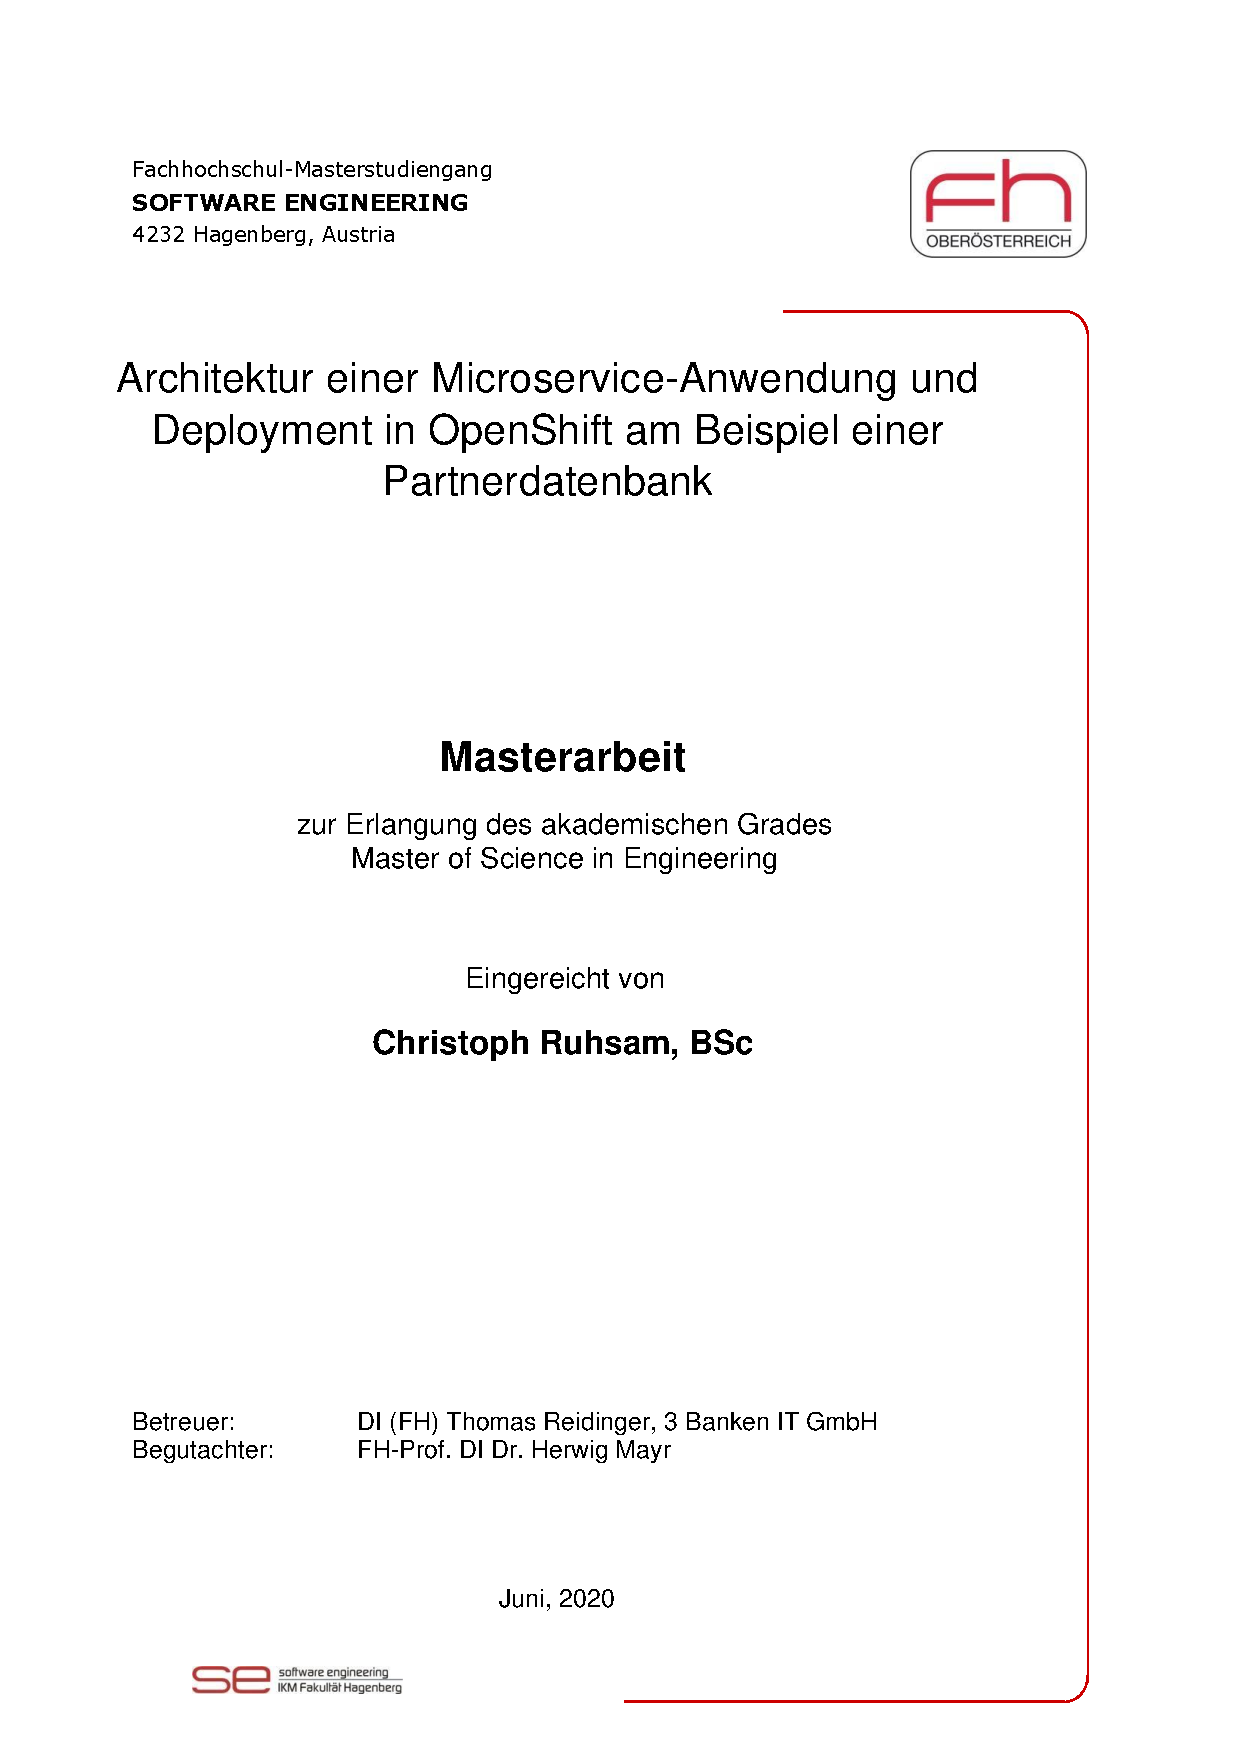
\includepdf[pages={1,2}]{title.pdf}
%\maketitle
\tableofcontents
\listoffigures

%\chapter{Preface}






 	% preface is optional
\chapter{Kurzfassung}

\begin{german}
An dieser Stelle steht eine Zusammenfassung der Arbeit, Umfang
max.\ 1 Seite. 
...
\end{german}
\chapter{Abstract}
An Enterprise Service Bus (ESB) is a crucial part of an enterprise, which connects the enterprise to its partners, customers, and other branches. The appearance of containerization, cloud services, and the microservice architecture have provided new possibilities for implementing and running an ESB. But, an ESB is commonly used by large conservative enterprises, which don't adapt new technologies fast, and wait until a new technology has proven itself. Especially the cloud is something the industry denied to use for a long time, because of the fact, that the infrastructure and data are managed and maintained by external service providers. \\ 

These days, we live in the so called cloud age, whereby global enterprises like Red Hat or Amazon provide cloud services such as Platform as a Service (PaaS), which can scale with the business. Enterprises start to consider to move their ESB installations to the cloud to profit from the cloud service provided features. Moving an ESB to the cloud will be a long term process for an enterprise, because the established processes for development, running, and managing the ESB will have to change. \\

This thesis has the goal to give the reader an overview of the cloud related concepts and technologies such as, Infrastructure as Code (IaC) and Docker, which are the base for cloud services. The implemented ESB prototype,  is  available at \url{https://github.com/cchet-thesis-msc/prototype}, and shows how an ESB could be implemented on a PaaS platform. \\




%%%----------------------------------------------------------
\mainmatter          			% main part (arabic page numbers)
%%%----------------------------------------------------------

\chapter{Einleitung}
In diesem Kapitel wird die grundsätzliche Motivation zu Microservices und Cloudtechnologien gezeigt. Auch das Ziel der Partnerdatenbank, ein Leitfaden, sowie die Gliederung der Schrift werden in diesem Abschnitt beschrieben.

\section{Motivation zur Architektur von Microservices}
Enterprise-Softwarearchitektur entwickelt sich durch neue Architekturdesigns immer weiter. Paradigmenwechsel im Technologieumfeld und der Wunsch nach besseren und schnelleren Applikationen tragen zur Entwicklung der Architektur bei \cite{MicroservicesForTheEnterprise}.

Microservices wurden als Architekturdesign sehr gut aufgenommen und sind nun weit verbreitet. Sie tragen zur schnelleren und sichereren Entwicklung der Erstellung von Software bei. Die Microservice-Architektur stärkt den Bau von Softwaresystemen als Sammlung von unabhängigen und autonomen Services. Microservices werden durch lose Kopplung unabhängig voneinander entwickelt, deployt und skaliert. Durch den Zusammenschluss aller Microservices entsteht eine gemeinsame Applikation \cite{MicroservicesForTheEnterprise}.

Ein Microservice ist dabei eine Implementierung einer wohldefinierten Businessfunktion und ist über ein Netzwerk erreichbar. Microservices weisen ein wohldefiniertes Interface auf. Die Aufrufer des Microservice verlassen sich auf das Interface und kümmern sich nicht um die dahinterliegende Implementierung \cite{MicroservicesForTheEnterprise}.

Eines der Kernkonzepte von Microservices ist, dass die Architektur der Services auf Businesszwecke abgestimmt und definiert sein muss. Ein Microservice fokussiert lediglich auf einen Businessaspekt. Ist dies nicht der Fall, muss das Microservice in weitere Microservices zerlegt werden \cite{MicroservicesForTheEnterprise}.

Durch das unabhängige Deployment der Microservices kann eine unabhängige Skalierung ermöglicht werden. Da sich Businessfunktionen bezüglich der Menge an Netzwerkverkehr unterscheiden, können einzelne Microservices einfach hochskaliert werden, ohne weitere Microservices hochskalieren zu müssen, die ohnehin wenig Netzwerkverkehr aufweisen. Dies spart Ressourcen und ist gerade beim Einsatz von Cloudtechnologien ein entscheidender Faktor \cite{MicroservicesForTheEnterprise}.


\section{Motivation zum Einsatz von Cloudtechnologien}
Cloudtechnologien präsentieren einen neuen Weg Applikationen zu teilen und zu deployen. Sie bieten Usern die Möglichkeit, Information im Internet gemeinsam und gleichzeitig zu bearbeiten, anzusehen und zu teilen. Die Cloud selbst ist ein Netzwerk von Datencentern, wobei jedes Datencenter eine Fülle von Rechnern aufweist, die gemeinsam interagieren. Die Cloud ist auch ein Set von Services, das eine skalierbare und anpassbare, billige Infrastruktur für Entwickler und Enduser bereitstellt. Auf diese Infrastruktur kann jederzeit sehr einfach zugegriffen werden \cite{CloudComputing}.

Cloudanbieter stellen den Usern einen großen Pool an Ressourcen zur Verfügung mit der Möglichkeit, diese Ressourcen sehr einfach zu managen. Die wichtigsten Kernpunkte und Vorteile von Cloud Computing umfassen \cite{CloudComputing}:
\begin{itemize}
	\item \textbf{Agilität}: Agilität hilft beim schnellen und billigen Zurverfügungstellen von Ressourcen.
	\item \textbf{Standortunabhängigkeit}: Auf Ressourcen kann von überall zugegriffen werden.
	\item \textbf{Teilbarkeit}: Ressourcen werden von einem großen Pool an Usern geteilt.
	\item \textbf{Zuverlässigkeit}: Ressourcen sind hoch verfügbar.
	\item \textbf{Skalierbarkeit}: Dynamische Zurverfügungstellen von Daten hilft bei der Vermeidung von Bottleneck-Szenarien.
	\item \textbf{Wartung}: User haben weniger Aufgaben bei Upgrades und beim Management von Ressourcen. Diese Aufgaben übernimmt der Cloud Provider.
\end{itemize}

Cloud Computing setzt dabei auf zwei wichtige Techniken \cite{CloudComputing}:
\begin{enumerate}
	\item \textbf{Serviceorientierte Architekturen}: Serviceorientierte Architekturen beinhalten ein Set von Designprinzipien, die während der Softwareentwicklung und der Softwareintegration genutzt werden. Das Deployment von serviceorientierten Architekturen bietet ein lose gekoppeltes Set an Services, die über mehrere Businessgrenzen hinweg kommunizieren können.
	\item \textbf{Virtualisierung}: Das Konzept der Virtualisierung befreit den User von Ressourcenkäufen und aufwändigen Installationen. Die Cloud bringt die Ressourcen zum User. Virtualisierung umfasst Hardware, Speicher, Speicherzugriff, Software, Daten und Netzwerke. Virtualisierung ist im Cloudumfeld zu einem unverzichtbaren Bestandteil geworden. Durch Virtualisierung können mehrere Applikationen am selben Server laufen und gemeinsam Ressourcen teilen. Durch verschiedene Host Operating Systeme ist die Konfiguration einiger Applikationen sehr umständlich. Auch dieses Problem löst Virtualisierung durch einfache Konfiguration und Aggregation von Ressourcen. Auch das schnelle Recovery-Management ist ein großer Pluspunkt bei Virtualisierung und bei Cloudtechnologien.
\end{enumerate}

Durch diese Vorteile sind Cloudtechnologien in den letzten Jahren immer wichtiger und populärer geworden. Ein Anbieter einer Software kann sich heutzutage Downtimes seines Produkts nicht mehr leisten. Viele Kunden wechseln durch die Fülle an Angeboten schnell zum Konkurrenten. Cloud Provider bieten durch Service Level Agreements meist eine Verfügbarkeit von über 99\%. Auch deshalb hosten viele Softwarefirmen nicht mehr selbst, sondern deployen diese in Cloudsysteme \cite{CloudComputing}.

\section{Zielsetzung der Implementierung der Partnerdatenbank}
Bei der 3 Banken IT GmbH gibt es zusätzlich zu den Kunden, wie der BKS Bank, der Oberbank und der BTV Vier Länder Bank, auch Partner, wie z.B. die FH Oberösterreich Campus Hagenberg oder die JKU Linz. Diese Partner werden aktuell in verschiedenen Datenquellen geführt.
Die aktuellen Datenquellen der 3 Banken IT GmbH bestehen aus:
\begin{itemize}
	\item \textbf{FiPe-/Docsis-Liste} Sobald Dokumente gescannt werden, wird in der Firmenpersonalliste der Partner mit Kürzel, Name und laufender Nummer erfasst. Dadurch kann im Dokumentenmanagementsystem Docsis auf das Kürzel und die laufende Nummer aus der FiPe-Liste zugegriffen werden.
	\item \textbf{SAP}: Sobald Rechnungen eintreffen, wird der Partner im SAP als Kreditor mit Name, Adresse und laufender Nummer aus der FiPe-Liste und Bankverbindungen erfasst.
	\item \textbf{Art28\_Verträge\_Fernwartungszugänge\_VPE}: Diese Daten werden ab der Angebotsanfrage/Ausschreibung benötigt.
	\item Ansprechpersonen mit \textbf{Kontaktdaten} von den Anwendungsverantwortlichen bei den einzelnen Mitarbeitern.
\end{itemize}

Ziel der Partnerdatenbank ist die Ablöse der Art28\_Verträge\_Fernwartungszugänge\_VPE und der FiPe-Liste.
Weitere funktionale Anforderungen werden wie folgt definiert:
\begin{itemize}
	\item Es können Unternehmen als Partner angelegt werden.
	\item Zu diesen Unternehmen können Kontaktpersonen hinzugefügt werden.
	\item Zu Kontaktpersonen gehören verschiedene Links im Docsis. Auch diese werden in der Applikation angezeigt.
	\item Die Ersterfassung eines Partners ist durch jeden Mitarbeiter möglich.
	\item Es besteht die Möglichkeit einen Kontakt als privat oder öffentlich zu markieren. Dies ist wichtig, wenn jemand seine Visitenkarten darin verwaltet.
	\item Der Basiseintrag einer Firma ist generell öffentlich. Nur für Kontaktpersonen kann ein privater Status angegeben werden.
\end{itemize}
Zu den nicht-funktionalen Anforderungen zählen:
\begin{itemize}
	\item eine Microsoft SQL Server Datenbank,
	\item Spring-Boot als Backendtechnologie,
	\item Angular als Frontendtechnologie,
	\item ein rollenbasierter Login mit Username und Passwort,
	\item das Backend als Microservice-Architektur,
	\item eine Infrastruktur zum Deployment in OpenShift.
\end{itemize}

Weiters sollen zusätzliche Tools eingebunden werden, die bei der Entwicklung von Microservices und dem Deployment in OpenShift helfen. Zu diesen Tools zählen:
\begin{itemize}
	\item \textbf{Jenkins} dient für automatisierte Test-, Build- und Deployment-Pipelines.
	\item \textbf{Spring-Retry} dient zur Fehlerbehandlung speziell bei Microservices.
	\item \textbf{Swagger} dient zur REST-Schnittstellenbeschreibung.
	\item \textbf{Jaeger} dient zum Tracing von Serviceaufrufen.
	\item \textbf{Docker} dient zur Containerisierung der einzelnen Services.
	\item \textbf{Fabric8} dient zum Deployment der Services in OpenShift.
\end{itemize}

Durch die Anwendung dieser Tools, der Microservice-Architektur und dem Deployment in OpenShift soll der 3 Banken IT GmbH ein Prototyp einerseits für die Weiterentwicklung der Partnerdatenbank, andererseits eine Schablone für weitere Anwendungen geboten werden.

\section{Ziel des Deployments der Partnerdatenbank in OpenShift}
Cloud Services, wie OpenShift, weisen grundsätzlich folgende drei Charaktereigenschaften auf:
\begin{enumerate}
	\item Nutzer können eine große Anzahl an Ressourcen jederzeit nutzen.
	\item Cloud Services sind elastisch. Ein Nutzer kann jederzeit so viele Ressourcen wie möglich und so viele wie nötig nutzen.
	\item Das Service wird gänzlich vom Provider gemanagt. Die Nutzer benötigen lediglich Internetzugang und Rechner, um die Services aufzurufen. 
\end{enumerate}

Durch die Nutzung von OpenShift und das Deployment der Anwendung in OpenShift muss die 3 Banken IT GmbH keine eigenen Ressourcen zum Hosten der Anwendung bereitstellen. Der Cloud Provider kümmert sich um die Aufrechterhaltung der Infrastruktur.

OpenShift ist eine Open-Source Platform-as-a-Service Plattform. OpenShift bietet automatische Installation, Upgrades und Lifecycle-Management des gesamten Container Stacks auf jeder Cloud Plattform. Zum Container Stack gehören das Betriebssystem, Kubernetes, Cluster Services und Applikationen \cite{OpenShiftOnline}.

OpenShift hilft Teams auch beim schnellen und agilen Erstellen von Anwendungen. Dadurch, dass Befehle in der Dev-Stage dieselben wie in der Production-Stage sind, können Entwickler noch sicherer und einfacher Applikationen entwickeln. Gerade bei Software für Banken ist die Sicherheit wesentlich.

Auch dadurch, dass die 3 Banken IT GmbH bereits Applikationen in OpenShift deployt, ist die Wahl der Cloud-Infrastruktur der Partnerdatenbank auf OpenShift gefallen.

\section{Leitfaden und Gliederung der Schrift}
Die Schrift gliedert sich in folgende neun Kapitel:
\begin{enumerate}
	\item \textbf{Einleitung}: In diesem Kapitel wird die Motivation von Microservices und Cloudtechnologien beschrieben. Auch die Zielsetzung der Implementierung der Partnerdatenbank, sowie das Ziel des Deployments in OpenShift wird erklärt.
	\item \textbf{Serviceorientierte Architektur und Microservices}: In diesem Kapitel wird die Abgrenzung serviceorientierter Architekturen zu Microservices beschrieben. Auch ein Vergleich mit monolithischen Architekturen und die Charakteristiken sowie die Vor- und Nachteile von Microservices werden gezeigt.
	\item \textbf{Containerisierung mit Docker}: In diesem Kapitel wird die Notwendigkeit der Containerisierung von Cloud-Applikationen am Beispiel von Docker gezeigt.
	\item \textbf{OpenShift}: In diesem Kapitel werden OpenShift sowie die Container-as-a-Service-Plattform Kubernetes, auf welcher OpenShift aufsetzt, gezeigt.
	\item \textbf{Partnerdatenbank}: In diesem Kapitel werden der Grundaufbau und Zweck der Partnerdatenbank, sowie die Beschreibung der Backends und des Frontends gezeigt.
	\item \textbf{Implementierung der Partnerdatenbank}: In diesem Kapitel werden die Implementierung der Partnerdatenbank und auch die Integration der Tools, wie Jenkins, Swagger oder Jaeger, gezeigt.
	\item \textbf{Evaluierung der Anwendung}: In diesem Kapitel werden die Architekturevaluierung, Evaluierung des Frontends und Whitebox- sowie Blackbox-Tests gezeigt.
	\item Abschließend gibt der Verfasser eine \textbf{Zusammenfassung} und einen Ausblick über die weitere Entwicklung der Partnerdatenbank.
\end{enumerate}
\chapter{Serviceorientierte Architektur und Microservices}
Das folgende Kapitel behandelt Microservices, ihre Vor- und Nachteile und die Abgrenzung zu serviceorientierten Architekturen sowie die Unterschiede zu monolithischen Architekturen.
\section{Definition und Abgrenzung}
Im Folgenden werden die Definition von Microservices und die Abgrenzung zu serviceorientierten Architekturen beschrieben.

\subsection{Definition von Microservices}
Microservices sind ein Ansatz, um große Softwarearchitekturen in kleine, konsistente, voneinander klar abgegrenzte Services zu zerlegen. Diese Services sind isoliert und kommunizieren miteinander \cite{MicroservicesForJavaDevelopers}.

Microservices werden typischerweise von kleinen Teams implementiert, gebaut und deployt. Diese kleinen Services sind so autonom, dass das Team, welches für den Service zuständig ist, die Implementierungsdetails ändern kann, ohne großen Einfluss auf das gesamte restliche System zu haben.
Jedes Team ist selbst für sein Service verantwortlich. Das Team muss für die Aufgabenstellung die richtige Technologie wählen, das Service deployen und managen und etwaige Fehler beheben.
Bei Microservice-Architekturen kann die Abgrenzung der verschiedenen Services ganz klar definiert werden. \cite{MicroservicesForJavaDevelopers} Dies hilft, um \cite{MicroservicesForJavaDevelopers}:
\begin{enumerate}
	\item \label{SOA:Abgrenzung:logik} die Logik des Services einfach zu verstehen, ohne den Kontext der gesamten Applikation kennen zu müssen,
	\item \label{SOA:Abgrenzung:bauen} den Service schnell lokal bauen und ausführen zu können,
	\item \label{SOA:Abgrenzung:technologie} die richtige Technologie für ein Problem zu nützen,
	\item \label{SOA:Abgrenzung:testen} den Service einfach und schnell testen zu können, ohne die gesamte Applikation dabei hochfahren zu müssen,
	\item \label{SOA:Abgrenzung:release} schnellere Releasezeiten zu ermöglichen,
	\item \label{SOA:Abgrenzung:skalierung} schnellere horizontale Skalierung zu ermöglichen,
	\item \label{SOA:Abgrenzung:belastbarkeit} die Belastbarkeit des Systems zu verbessern.
\end{enumerate}

Die oben angeführten Punkte werden im Folgenden näher ausgeführt \cite{MicroservicesForJavaDevelopers}:

\textbf{\ref{SOA:Abgrenzung:logik} Logik}: Jedes einzelne Microservice sollte nur einen Teil der gesamten Anwendung ausmachen. Ein Microservice deckt meist nur einen Geschäftsfall der gesamten Businesslogik ab. Dieser Geschäftsfall ist für sich einfacher zu verstehen als das gesamte System. Kommt ein neuer Entwickler in das Team, muss er sich nur in den Code des Microservice, an dem er arbeitet, einlesen und muss nicht das gesamte System verstehen.

\textbf{\ref{SOA:Abgrenzung:bauen} Bauen und Ausführen}: Muss bei einem neuen Feature die gesamte Anwendung gebaut, deployt und ausgeführt werden, ist dies sehr aufwändig und kostet sehr viel Zeit. Ein Microservice hingegen steht für sich selbst und kann einfach lokal gestartet und getestet werden. Dies erleichtert dem Entwickler die Arbeit und spart Zeit.

\textbf{\ref{SOA:Abgrenzung:technologie} Technologie}: Meist werden für bestimmte Geschäftsfälle verschiedene Technologien benötigt. Ist die gesamte Businesslogik in einem Monolithen abgebildet, kann lediglich eine Technologie eingesetzt werden. Ist aber beispielsweise für einen bestimmten Geschäftsfall Machine Learning nötig, ist eventuell Java die falsche Lösung und man setzt lieber auf Python.
Microservices sind unabhängig voneinander und kommunizieren meist durch REST oder SOAP (siehe dazu Abschnitt \ref{subsec: AbgrenzungServiceorientierte}) miteinander. Dadurch kann in jedem Service die gewünschte Technologie eingesetzt werden.

\textbf{\ref{SOA:Abgrenzung:testen} Testen}: Ähnlich zu \ref{SOA:Abgrenzung:bauen}, wo das Bauen und Ausführen eines Microservice beschrieben wird, kann ein Service auch unabhängig vom gesamten System getestet werden.

\textbf{\ref{SOA:Abgrenzung:release} Releasezeiten}: Heutzutage müssen neue Features schnell ausgeliefert werden, ansonsten ist womöglich der Konkurrent schneller und man verliert Kunden. Muss bei einem neuen Release das gesamte System neu deployt werden, sind damit verschiedenste Risiken verbunden. Wird z.B. ein fehlerhafter Code deployt, stürzt der gesamte Monolith ab. Bei Microservices ist in dieser Zeit lediglich das neu deployte Service nicht verfügbar.

\textbf{\ref{SOA:Abgrenzung:skalierung} Skalierung}: Hat man ein monolithisches System und möchte einen neuen Geschäftsfall implementieren, muss dieser in das bestehende System eingeflochten werden, was dazu führen kann, dass ein bestehender Code nicht mehr so funktioniert wie gewollt.
Bei einer Microservice-Architektur wird ein neues Service für diesen Geschäftsfall angelegt und bestehender Code nicht oder kaum für Aufrufe des neuen Service geändert.

\textbf{\ref{SOA:Abgrenzung:belastbarkeit} Belastbarkeit}: Fällt ein Service aus, heißt das nicht, dass das gesamte System nicht mehr verfügbar ist. Teile des Systems können meist ohne Probleme weiterverwendet werden.



\subsection{Abgrenzung serviceorientierter Architekturen und Microservices}
\label{subsec: AbgrenzungServiceorientierte}
Microservices und serviceorientierte Architekturen gehören beide zu den service-basierten Architekturen. Das heißt, dass beide Architekturen einen großen Schwerpunkt auf Services als primäre Architekturkomponenten legen. Obwohl Microservices und serviceorientierte Architekturen sehr unterschiedliche Muster aufweisen, haben sie auch viele Gemeinsamkeiten \cite{MicroservicesVSSOA}.

Alle serviceorientierten Architekturen sind verteilte Architekturen. Die Servicekomponenten werden über Remote-Protokolle, wie beispielsweise Representational State Transfer (REST), Simple Object Access Protocol (SOAP) oder Java Message Service (JMS) angesprochen.
Beide bieten viele Vorteile im Vergleich zu monolithischen und schichten-basierten Architekturen. Sie bieten höhere Skalierbarkeit, losere Kopplung zwischen den Services und bessere Kontrolle über Entwicklung, Tests und Deployment. Komponenten in einer verteilten Anwendung tendieren mehr dazu, in sich geschlossen zu sein und bieten daher besseres Änderungsmanagement und einfachere Wartung, was zu mehr Flexibilität und zu robusteren Anwendungen führt.
Diese Architekturen führen auch zu loser gekoppelten und modulareren Anwendungen. 
Modularität bedeutet das Kapseln einzelner Teile der Anwendung in abgeschlossene Services, die dadurch individuell designt, entwickelt, getestet und deployt werden können, ohne großen Einfluss auf andere Services zu nehmen \cite{MicroservicesVSSOA}.

Sowohl bei Microservices als auch bei serviceorientierten Architekturen müssen \textit{Service Contracts} vereinbart werden. Service Contracts werden zwischen einem Service und einem Servicekonsumenten (Client) vereinbart. Dadurch wird das Format der eingehenden und ausgehenden Daten spezifiziert (z.B. XML, JavaScript Object Notation [JSON], Java Object, etc.) \cite{MicroservicesVSSOA}. 

Microservice-Teams bestehen meist aus maximal sieben Personen. Das Team muss die Entwicklung, das Deployment und den Betrieb des Service alleine bewältigen. Je größer das Team, desto höher ist der Kommunikationsaufwand. Jedes Teammitglied sollte die gesamte Codebasis überblicken und warten können. Zu große Teams sind meist ein Indikator dafür, dass das Service aufgesplittet werden sollte \cite{MicroservicesVSSOA}.

Serviceorientierte Architekturen sind eher für große, komplexe Enterprise-Systeme geeignet, die eine Interaktion mit vielen heterogenen Applikationen und Services benötigen. Für Anwendungen, die viele Komponenten benötigen und von mehreren Services geteilt werden, sind serviceorientierte Architekturen passend.
Für Applikationen mit einem wohldefinierten Arbeitsablauf und wenig gemeinsam geteilten Komponenten, wie z.B. Security-Komponenten, sind Microservice-Architekturen sinnvoll.
Microservice-Architekturen sind besser geeignet für kleine, wohl definierte, web-basierte Systeme, als für groß skalierbare Enterprise-Systeme. Die fehlende Middleware ist ein Faktor, weshalb Microservice-Architekturen nicht oder schlecht für komplexe Businessanwendungen geeignet sind. Microservices sollten dort eingesetzt werden, wo sich die Businesslogik auf kleine, abstrahierte Geschäftsfälle herunterbrechen lässt \cite{MicroservicesVSSOA}.

Microservices und serviceorientierte Architekturen sind auch bezüglich Teilen von Komponenten sehr unterschiedlich. Serviceorientierte Architekturen basieren auf dem Prinzip \textit{share-as-much-as-possible}, wohingegen Microservices auf dem Prinzip \textit{share-as-little-as-possible} basieren.
Angenommen, ein großes Warenhaus benötigt zum Verwalten der Einkäufe und Verkäufe jeweils ein \textit{Bestellservice}. Bei serviceorientierten Architekturen, wie in Abbildung \ref{fig:SOA_Bestellservice} zu sehen, würde man dazu das Bestellservice einmal implementieren und die Einkaufs- und Verkaufskomponente teilen sich dieses Service. Das Bestell-Service selbst muss in diesem Fall wissen, welche Aktionen es bei den verschiedenen Anfragen ausführen muss.
Obwohl das \textit{share-as-much-as-possible}-Prinzip das Problem der Codeduplizierung löst, ist damit eine enge Kopplung von Businesskomponenten verbunden und erhöht das Risiko bei Änderungen. Angenommen, man ändert den Code im Business-Service, ist diese Änderung schwer zu testen, da das Service global verfügbar ist und je nach Aufruf andere Aktionen auslöst \cite{MicroservicesVSSOA}.

\begin{figure}[H]
	\begin{center}
		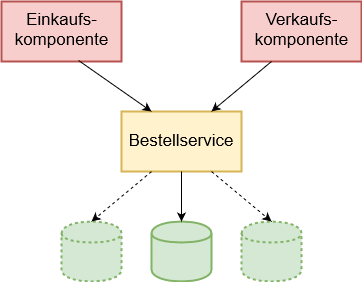
\includegraphics[scale=0.80]{SOA_Bestellservice.png}
		\caption[Serviceorientierte Architektur - Bestellservice]{Serviceorientierte Architektur - Bestellservice \cite{MicroservicesVSSOA}}
		\label{fig:SOA_Bestellservice}
	\end{center}
\end{figure}

Microservices basieren auf dem Konzept \textit{share-as-little-as-possible} und verstärken dadurch das Domain-driven Designkonzept \textit{Bounded Context}. Microservices sind lose gekoppelt und agieren daher als einzelne geschlossene Einheit mit wenig Abhängigkeiten. Es gibt lediglich ein wohldefiniertes Interface und wohldefinierte Vereinbarungen nach außen. 
Realistischerweise wird es immer gemeinsam geteilte Services geben, auch in Microservice-Architekturen, z.B. Sicherheits- oder Infrastrukturservices. Serviceorientierte Architekturen maximieren das Teilen von Komponenten, wohingegen Microservice-Architekturen das Teilen durch den klar definierten Bounded Context minimieren \cite{MicroservicesVSSOA}.

Es gibt viele Vorteile, die das Verstärken des Bounded Context bringt. Die Wartung der Services wird wegen der geringeren Abhängigkeiten weitaus einfacher. Dies erleichtert auch das Ändern und Weiterentwickeln des Services. Auch das Deployment gestaltet sich dadurch um einiges einfacher, da weniger Code zu deployen ist und es weniger Risiken gibt, andere Bereiche des gesamten Systems zu brechen. Dies fördert auch die Robustheit des gesamten Systems \cite{MicroservicesVSSOA}.


\section{Vergleich mit monolithischer Architektur}
Microservices und Monolithen sind sehr unterschiedliche Designstrategien, um eine Anwendung zu entwickeln. Beide Strategien haben ihre Vor- und Nachteile. Die Strategie sollte deshalb mit Bedacht gewählt werden. Die monolithische Architektur ist derzeit noch der Standardweg,  eine Applikation zu entwickeln \cite{FowlerDSM}.

Im Folgenden werden die wichtigsten Unterschiede von monolithischen und von Microservice-Architekturen beschrieben \cite{MonolithVSMicroservices}.

\subsection{Wartung}
Microservices sind viel einfacher zu warten, da sich die Komplexität eines Services in Grenzen hält. Microservices sind modulare und unabhängige Services. Neue Entwickler können sich in die Codebasis schneller einlesen und schneller neue Features implementieren als bei monolithischen Architekturen.

Ein Monolith besteht aus einer Codebasis, in der alle Geschäftsfälle abgedeckt sind. Wird ein neues Feature hinzugefügt, wird es dabei in die bestehende Codebasis eingewebt. 
Dies erhöht die Komplexität des Codes und erschwert die Entwicklung und Wartung.
Neue Entwickler müssen sich in die gesamte Codebasis und in den gesamten Workflow einlesen, um neue Features entwickeln zu können.

\subsection{Deployment}
Ein kontinuierliches Deployment gestaltet sich bei Monolithen sehr schwierig, da der Monolith immer größer und komplexer wird. Zudem muss immer der gesamte Monolith deployt werden, auch wenn lediglich wenig Codestücke geändert wurden. Dies ist natürlich sehr zeitaufwändig, aber auch gefährlich. Wird ein fehlerhafter Code deployt, bringt dieser den gesamten Monolith zum Stillstand.

Bei Microservices hingegen wird die Codebasis in kleine, überschaubare Services unterteilt, die einzeln und jederzeit schnell deployt werden können. Wird bei Microservice-Architekturen ein fehlerhafter Code deployt, ist es möglich, dass andere Teile des gesamten Systems noch ohne Probleme laufen.

\subsection{Tests}
Auch beim Testen eines Monolithen werden die große Codebasis und die vielen verschiedenen Anwendungsfälle zum Problem. Das Testen aller Szenarien bei einer derart großen Codebasis wird dabei schnell unübersichtlich.

Bei Microservices kann durch den Bounded Context jede Komponente individuell getestet werden. Dies erleichtert das Testen eines jeden Services ungemein und verringert zusätzlich die Fehleranfälligkeit eines Systems.

\subsection{Startup-Zeit}
Bei monolithischen Architekturen wird der gesamte Monolith hochgefahren. Je komplexer und größer dieser wird, desto mehr steigt die Startzeit.

Die Startzeit bei Microservices ist viel schneller, da jedes Service einzeln hochgefahren werden kann. Werden alle Services gemeinsam gestartet, bringt dies bezüglich der Startzeit wieder wenig.

\subsection{Technologie}
Ein Monolith wird in einer Programmiersprache entwickelt und greift meist nur auf eine Datenbank zu. Neue Technologien können nicht bzw. nur sehr umständlich hinzugefügt werden. Die Einarbeitungszeit gestaltet sich jedoch bezüglich Technologie einfacher, da nur eine Sprache zum Einsatz kommt und neue Entwickler nur diese beherrschen müssen.

Mit Microservices können Entwickler die Technologie jedes Services selbst wählen. Da Microservices so klein und überschaubar sind, können diese schnell ersetzt werden und es kann dadurch immer die aktuellste Version oder Technologie verwendet werden.

\subsection{Skalierbarkeit}
Microservices können einfach skaliert werden. Platform-as-a-Service-Plattformen, wie OpenShift, bieten eine einfache Möglichkeit, Services je nach Bedarf hoch- und runterskalieren zu können.

Einen komplexen Monolithen zu skalieren gestaltet sich sehr schwierig. Zum Beispiel wird ein kontinuierliches Deployment mit vielen Entwicklern und einer sehr großen Codebasis sehr kompliziert.


\section{Charakteristiken}
Im Folgenden werden die wichtigsten Charakteristiken von Microservices beschrieben, die auch für serviceorientierte Architekturen gelten \cite{SpringMicroservices}.

\subsection{Service-Vereinbarung}
Microservices werden durch wohldefinierte Service-Vereinbarungen beschrieben. Zum Datenaustausch kann z.B. REST oder SOAP verwendet werden. Als Markup-Sprache kann JSON, XML oder auch YAML eingesetzt werden. In der Welt der Microservices wird meist die Kombination von REST und JSON eingesetzt. Es gibt aber mehrere Möglichkeiten zur Definition von Service-Kontrakten. JSON Schema, WADL, Swagger und RAML sind nur ein paar wenige Beispiele.

\subsection{Lose Kopplung}
Microservices sind unabhängig und lose gekoppelt. Meist akzeptieren Microservices ein Event als Input und reagieren darauf erneut mit einem Event. Nachrichten, HTTP und REST werden häufig zur Interaktion zwischen den einzelnen Services eingesetzt. Nachrichten-basierte Endpunkte bieten dabei ein höheres Level an Entkopplung.

\subsection{Service-Abstraktion}
Service-Abstraktion bei Microservices ist nicht nur die abstrahierte Realisierung des Service, sondern bietet auch eine komplette Abstraktion von allen Bibliotheken und Umgebungsdetails.

\subsection{Wiederverwendung}
Microservices sind wiederverwendbare Business-Services. Sie werden von mobilen Geräten, Desktop-Anwendungen und auch anderen Microservices verwendet.

\subsection{Zustandslosigkeit}
Wohl-designte Microservices sind zustandslos und teilen sich nichts. Wird ein gemeinsamer Zustand in verschiedenen Services benötigt, wird dieser meist in einer Datenbank abgebildet.

\subsection{Interoperabilität}
Services sind durch Standardprotokolle und Nachrichtenaustausch-Standards interoperabel. Nachrichtenaustausch, HTTP und REST werden zum Nachrichtentransport verwendet. Eine Kombination aus REST und JSON ist die populärste Methode zum Entwickeln von interoperablen Services. Wird weitere Optimierung benötigt, kommen auch andere Protokolle, wie RabbitMQ, Avro, Zero MQ oder Protocol Buffers zum Einsatz. Der Einsatz dieser Protokolle kann dabei aber auch die Interoperabilität der Services einschränken.

\subsection{Zusammensetzung}
Microservices sind zusammensetzbar. Dies wird durch Service-Orchestrierung und Service-Choreografie erreicht. Service-Orchestrierung und Service-Choreografie sind zwei Designvarianten von Microservices. Auf diese wird im nächsten Abschnitt näher eingegangen.

\section{Designvarianten}
Im Folgenden werden die beiden Varianten \textit{Service Orchestrierung} und \textit{Service Choreografie} zum Design von Microservices vorgestellt.

\subsection{Service-Orchestrierung}
Bei der Service-Orchestrierung gibt es ein zentrales Kompositionsservice, dass das entsprechende Microservice aufruft und von diesem die Antwort erwartet. Diese Nachrichten können mittels HTTP oder Socketaufrufen durchgeführt werden. Wichtig hier ist, dass diese Aufrufe sowohl synchron als auch asynchron durchgeführt werden können. Das aufgerufene Microservice muss also nicht sofort antworten, sondern kann auch später mit der Antwort ein Event im Kompositionsservice auslösen.
In diesem Muster reden die Microservices nicht miteinander, sondern nur mit dem Kompositionsservice. Dabei muss jedoch nicht für jedes Microservice dasselbe Protokoll verwendet werden, z.B. kann das Kompositionsservice mit Service A über HTTP und mit Service B über das XML/RPC-Protokoll kommunizieren \cite{PracticalMicroservices}.

Wie in Abbildung \ref{fig:SOA_Orchestrierung} zu sehen, wird dabei das Kompositionsservice zur zentralen Autorität. Hier beginnt auch die gesamte Logik, was schlechtes Design für Microservices bedeutet. Die gesamte Logik im Kompositionsservice zu haben führt zu einer Fülle von Abhängigkeiten zwischen den Services. Z.B. kann die Logik sein, dass, wenn Service A antwortet, Service B danach aufgerufen werden muss. Dies führt zu Abhängigkeiten zwischen Service A und Service B \cite{PracticalMicroservices}.

Da das Kompositionsservice der zentrale Punkt der Anwendung ist, ist dieser auch die Schwachstelle. Dieses Service muss verfügbar sein, ansonsten steht die gesamte Anwendung still. Das Kompositionsservice ist der \textit{Single-Point-of-Failure} in dieser Architektur. Dies kann aber durch Tools und Cloud-basierte Lösungen, wie Skalierung oder Clustering, gelöst werden. Zusätzlich ist das Orchestrierungsmuster schwer zu implementieren. Hat man einen Entscheidungspunkt, wird es schwer, dem verteilten Design zu folgen \cite{PracticalMicroservices}.

\begin{figure}[H]
	\begin{center}
		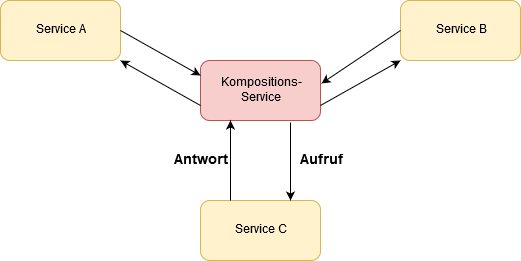
\includegraphics[scale=0.8]{SOA_Orchestration.png}
		\caption[Designvarianten - Service-Orchestrierung]{Varianten - Service-Orchestrierung \cite{PracticalMicroservices}}
		\label{fig:SOA_Orchestrierung}
	\end{center}
\end{figure}

\subsection{Service-Choreografie}
Anders als bei der Service-Orchestrierung ist bei der Service-Choreographie jedes Service in Koordination mit den anderen Services auf einen bestimmten Anwendungsfall zugeschnitten.
Service Orchestrierung repräsentiert die Kontrolle von einem einzelnen Standpunkt aus. Bei der Choreografie wird jedes Service in die Interaktion mit eingebunden \cite{PracticalMicroservices}. 

Wie in Abbildung \ref{fig:SOA_Choreographie} zu sehen, redet bei der Service Choreografie jedes Service nach Abschluss des Tasks mit einem anderen Service, um die nächste Aufgabe zu triggern. Dies kann in den Mustern \textit{one-to-one}, \textit{one-to-many} oder \textit{many-to-many} geschehen. Dies kann ebenfalls synchron oder asynchron durchgeführt werden. Idealerweise gibt es ein globales Protokoll, über das die Services miteinander kommunizieren. Meistens werden diese Aufrufe asynchron durchgeführt. Da es kein zentrales Service gibt, löst jedes Service ein Event nach Abschluss seines Tasks aus. Dies macht die Services unabhängig voneinander und fördert die lose Kopplung. Andere Services registrieren sich auf dieses Event und reagieren darauf, wenn es ausgelöst wird \cite{PracticalMicroservices}. 

Durch nachrichtenorientierte Kommunikation kann das Choreografiemuster sehr nützlich werden. Zwischen den Services wird eine Nachrichtenschlange implementiert. Dadurch wird das Loslösen, Hinzufügen und Entfernen von Services sehr einfach gelöst. Auch die ganze Reihe an Abhängigkeiten, die oft bei Choreografiemustern entstehen, wird dadurch gelöst. Service-Choreografie erhöht die Komplexität eines Systems. Jedes Service erzeugt und verarbeitet Nachrichten zur Laufzeit. Dadurch kann der exakte Stand einer Transaktion nicht herausgefunden werden \cite{PracticalMicroservices}.

\begin{figure}[H]
	\begin{center}
		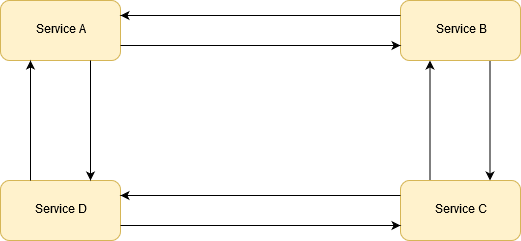
\includegraphics[scale=0.8]{SOA_Choreographie.png}
		\caption[Designvarianten - Service-Choreografie]{Varianten - Service-Choreografie \cite{PracticalMicroservices}}
		\label{fig:SOA_Choreographie}
	\end{center}
\end{figure}

\section{Vor- und Nachteile von Microservices}
Im folgenden Abschnitt werden die Vor- und Nachteile von Microservices behandelt.

\subsection{Vorteile von Microservices}
\subsubsection{Technologieunabhängigkeit}
Microservices werden als eigenständige Einheit betrachtet. Dadurch können die einzelnen Services verschiedene Technologien verwenden. Greift ein Service auf eine Datenbank zu und ein anderes Service führt Shell-Skripte aus, beeinflussen sich die beiden Services nicht und können jederzeit ausgetauscht werden, ohne Einfluss auf andere Services zu nehmen. Performanz ist in diesem Zusammenhang ebenfalls sehr wichtig. Wird eine Technologie zu langsam, kann sie ohne Probleme durch eine neue ersetzt werden \cite{Newman2015}.

\subsubsection{Skalierung}
Wie erwähnt, muss bei Monolithen die gesamte Software als Ganzes deployt und skaliert werden. Dies bedeutet viel Overhead. Bei Microservices können einzelne Teile hoch- und runterskaliert werden. Cloud-basierte Technologien, wie z.B. OpenShift, bieten diese Möglichkeit an. Es kann aber auch ein Microservice auf einer besseren Hardware laufen. Die anderen Services bleiben auf der billigeren Hardware. Monolithen müssten als Ganzes auf der besseren Hardware laufen. Dies verringert die Kosten der Skalierung bei Microservices drastisch \cite{Newman2015}.

\subsubsection{Austauschbarkeit}
Bei Microservices ist es sehr einfach, den bestehenden Code zu ändern oder auszutauschen. Da diese unabhängig sind, sind keine anderen Teile des Systems betroffen. Bei Monolithen stellt die Austauschbarkeit oft ein großes Risiko dar. Der Code ist oft sehr verwoben und kleine Änderungen haben große Auswirkungen \cite{Newman2015}.

\subsubsection{Entwicklerteam}
Entwickler greifen bei monolithischen Architekturen oft auf dieselben Teile des Codes zu. Bei Versionierungsprogrammen, wie Git oder Subversion, führt dies oft zu Konflikten.
Microservices können getrennt voneinander bearbeitet und der Code ohne Probleme zusammengefügt werden \cite{Newman2015}.


\subsection{Nachteile von Microservices}
\subsubsection{Hohe Latenzzeiten}
Microservices reden über das Netzwerk miteinander. Dieser Kommunikationsweg ist natürlich viel langsamer, als wenn diese in derselben JVM miteinander reden würden. Dies führt zu hohen Latenzzeiten. Diese müssen bei der Architektur von Microservices berücksichtigt werden \cite{Newman2015}.

\subsubsection{Wiederverwendbarkeit von Code}
Microservices sind unabhängige und eigenständige Einheiten. Sie haben im besten Fall keine Abhängigkeiten zueinander. Dadurch verringert sich die Wiederverwendbarkeit von Code. Dies führt auch zu einer Codeverdopplung. Wird dasselbe Codestück in zwei verschiedenen Services benötigt, muss es in beiden vorhanden sein \cite{Newman2015}.

\subsubsection{Deployment}
Jedes Service muss einzeln deployt werden. Dazu wird ein eigener Deployment-Prozess pro Service benötigt. Dies bedeutet Aufwand für die Entwickler und es muss eine eigene Infrastruktur geschaffen werden, was zusätzlich Kosten generiert \cite{Newman2015}.

\chapter{Containerisierung mit Docker}
Im Folgenden werden Docker, die Bestandteile von Docker und der Unterschied zwischen Virtualisierung und Containerisierung erklärt.
Anschließend wird auch die Notwendigkeit von Containerisierung für Cloud-Plattformen aufgezeigt.

\section{Docker}
Docker ist ein Container-Management-System, das es erleichtert, Linux Container zu managen. Docker erlaubt das Erstellen von Docker Images in virtuellen Umgebungen am lokalen PC. Auf diesen Umgebungen können Kommandos und Operationen ausgeführt werden. Diese Aktionen unterscheiden sich am lokalen PC nicht von den Aktionen am Produktivsystem. Dies hilft bei der Entwicklung lokal sowie beim Deployment auf der Produktivumgebung am Server, da die auszuführenden Kommandos dieselben sind \cite{MasteringDocker}.

\subsection{Komponenten von Docker}
Im Folgenden werden die Kernkomponenten von Docker beschrieben.

\subsubsection{Docker Engine}
Docker ist eine Client-Server Anwendung. Der Docker-Server wird auch als \textit{Docker Daemon} oder \textit{Docker Engine} bezeichnet. Bei der Installation von Docker werden eine Command Line Binary und eine RESTful API mitgeliefert, um mit dem Docker Daemon zu interagieren. Der Docker Daemon und der Docker Client können am selben Host laufen. Der lokale Docker Client kann aber auch mit einem Remote Docker Daemon verbunden werden.
Der Docker Daemon erzeugt und managt die Docker Container am Docker Host. Die Kommunikation des Docker Client mit dem Docker Daemon läuft über die von Docker bereitgestellte REST-API. \cite{TheDockerBook}

\subsubsection{Docker Images}
Docker Images sind die Bausteine im Docker System. Docker Container werden aus Docker Images gestartet. Docker Images sind mehrschichtig und werden schrittweise mittels einer Serie von Instruktionen erstellt.
Beispiele für solche Instruktionen sind:
\begin{itemize}
	\item eine Datei hinzufügen,
	\item einen Befehl im Container ausführen,
	\item einen Port öffnen.
\end{itemize}

Docker Images werden auch als \glqq Source Code\grqq{} für Container bezeichnet. Docker Images sind sehr portabel und können einfach verbreitet, gespeichert und aktualisiert werden \cite{TheDockerBook}. 

Die Instruktionen zum Bauen eines Docker Image werden in einem \textit{Dockerfile} beschrieben. Kommandos, Aufrufe von Scripts, das Setzen von Environment-Variablen, das Hinzufügen von Dateien und das Setzen von Rechten können alle im Dockerfile beschrieben werden. Im Dockerfile muss auch das Basisimage für den Build spezifiziert werden. Ein Dockerfile sieht beispielsweise wie in Listing \ref{lst:BSPDockerfile} dargestellt aus \cite{MasteringDocker}:

\begin{lstlisting}[language=docker, caption=Beispiel für ein Dockerfile, label={lst:BSPDockerfile}]
	FROM ubuntu:latest
	MAINTAINER Scott P. Gallagher <email@somewhere.com>
	
	RUN apt-get update && apt-get install -y apache2
	
	ADD 000-default.conf /etc/apache2/sites-available
	RUN chown root:root /etc/apache2/sites-available/000-default.conf
	
	EXPOSE 80
	CMD ["/usr/sbin/apache2ctl", "-D", "FOREGROUND"]
\end{lstlisting}

Dies sind typische Befehle, die in den meisten Dockerfiles zu finden sind. Im \textit{FROM}-Befehl wird das Basisimage, auf dem das Docker Image aufgebaut ist, definiert. Jede weitere Zeile fügt eine neue  Schicht im Docker Image hinzu. Mit dem Befehl:
\begin{lstlisting}[language=bash]
$ docker build <DOCKERFILE>
\end{lstlisting}
kann dieses Docker Image gebaut werden. Aus diesem Docker Image kann danach ein Docker Container erzeugt werden \cite{MasteringDocker}.

\subsubsection{Registries}
Die gebauten Docker Images werden in Registries gespeichert. Dabei gibt es zwei verschiedene Arten von Registries: \textbf{public} und \textbf{private}. Docker, Inc., verwaltet die public Registry, auch \href{https://hub.docker.com/}{Docker Hub} genannt. In der public Registry befinden sich auch bereits vordefinierte Docker Images für zum Beispiel eine MySQL-Datenbank oder einen Nginx Webserver.
Es kann auch eine eigene private Registry erstellt werden. Diese erlaubt das Speichern von Images, ohne dass von außen auf diese zugegriffen werden kann \cite{TheDockerBook}.

\subsubsection{Docker Container}
In Docker Containern können Applikationen und Services laufen. Docker Container werden aus Docker Images erstellt und können einen oder mehrere Prozesse enthalten. 
Ein Docker Container besteht aus \cite{TheDockerBook}:

\begin{itemize}
	\item einem gebauten Docker Image,
	\item einem Set von Standardoperationen,
	\item einer Umgebung zum Ausführen der Operationen.
\end{itemize}

Jeder Docker Container enthält ein Software Image, dass das Erstellen, Starten, Stoppen, Neustarten und Löschen des Docker Containers erlaubt. Docker kümmert sich dabei nicht um den Inhalt des Containers. Jeder Container, egal ob eine MySQL-Datenbank oder ein Nginx Webserver, wird gleich gestartet oder gelöscht.
Docker ist dabei unabhängig von der Umgebung in, der der Docker Container läuft. Es kann lokal am PC gebaut, in die public Registry hochgeladen werden oder der Container in der Cloud laufen. Dadurch kann mit Docker schnell ein Application Server, ein Message Bus oder ein Continous-Integration-Test erstellt und getestet werden \cite{TheDockerBook}.

\subsection{Unterschied zwischen Virtualisierung und Containerisierung}
\subsubsection{Virtualisierung}
Eine virtuelle Maschine, welche die Virtualisierung auf Hardware-Level repräsentiert, ist grundsätzlich ein komplettes Operating System, das in einem Host Operating System läuft. Dabei gibt es zwei Arten von \glqq Virtualization Hypervisors\grqq: \textbf{Type 1} und \textbf{Type 2}. Type 1 Hypervisors bieten Server-Virtualisierung auf Hardware-Level. Dabei gibt es kein traditionelles End-User Operating System.
Type 2 Hypervisors werden zur Desktop Virtualisierung verwendet. Die Virtualisierungs-Engine läuft dabei auf einem eigenen Operating System. Der größte Vorteil von virtuellen Maschinen ist, dass mehrere unterschiedliche Operating Systeme auf einem Host laufen können \cite{DevelopingWithDocker}.

Virtuelle Maschinen sind voll isoliert und daher sehr sicher. Sie enthalten jedoch alle Bestandteile, die ein Operating System aufweisen muss: Treiber, Systembibliotheken, etc.
Virtuelle Maschinen sind daher sehr schwergewichtig und ressourcenhungrig. Auch die Installation virtueller Maschinen ist sehr komplex und aufwändig. Um eine Applikation in einer virtuellen Maschine zu starten, muss der Hypervisor die virtuelle Maschine zuerst importieren und danach starten. Weiters können nur wenige virtuelle Maschinen auf einer einzelnen Maschine gestartet werden, da die Performanz mit jeder neuen virtuellen Maschine drastisch abnimmt \cite{DevelopingWithDocker}.

\subsubsection{Containerisierung}
Abbildung \ref{fig:DOC_DockerVSTraditional} zeigt einen der größten Vorteile von Docker. Docker benötigt kein neues Betriebssystem, sobald ein neuer Container gestartet wird. Dies verringert die Größe der einzelnen Container drastisch. Docker baut dabei auf den Linux Kernel des Host OS auf. Dies macht es möglich, jedes Linux OS als Host OS zu verwenden. Beispielsweise kann auf der linken App in der Abbildung auf der Dockerseite Red Hat laufen und auf der anderen Debian. Dazu muss weder Red Hat noch Debian auf dem Host installiert sein.
Docker Images werden dadurch so klein wie möglich gehalten. Sie sind dadurch sehr kompakt und einfach zu deployen \cite{MasteringDocker}.

Docker Container sind nicht nur vom darunterliegenden Operating System isoliert, sondern auch von anderen Docker Containern. Die Startzeiten von Docker Containern sind in der Regel durch den geringen Overhead sehr schnell. Docker Container ersetzen jedoch virtuelle Maschinen nicht ganz. Es muss vor der Entwicklung evaluiert werden, welches Vorgehen die beste Wahl ist. Auf der einen Seite gibt es völlig isolierte, sichere virtuelle Maschinen mit durchschnittlicher Performanz und auf der anderen Seite hoch performante, schnell deploybare Docker Container \cite{DevelopingWithDocker}.

\begin{figure}[H]
	\begin{center}
		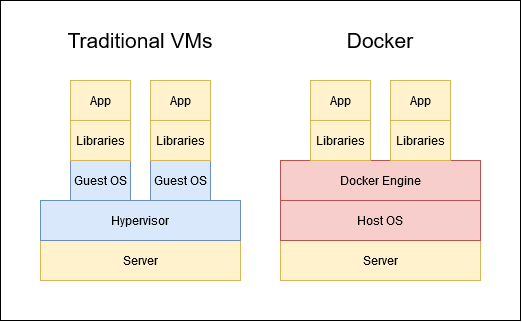
\includegraphics[scale=0.65]{DockerVSTraditional.png}
		\caption[Unterschied von traditionellen VMs zu Docker]{Unterschied von traditionellen VMs zu Docker \cite{MasteringDocker}}
		\label{fig:DOC_DockerVSTraditional}
	\end{center}
\end{figure}

\subsection{Vorteile von Docker}
In diesem Abschnitt werden die Vorteile von Docker und Containerisierung im Gegensatz zu virtuellen Maschinen und Virtualisierung beschrieben.

\subsubsection{Schnelligkeit und Größe}
Docker Container können schnell und einfach erstellt und wieder gelöscht werden. Docker teilt sich nur den Kernel mit dem Operating System. Auch Schichten von Docker Images können wiederverwendet werden. Dies führt zu sehr leichtgewichtigen Docker Containern. Die Resultate sind schnelles Deployment, einfache Migration und kurze Startzeiten \cite{DevelopingWithDocker}.

\subsubsection{Reproduzierbarkeit und portable Builds}
Docker erlaubt das Deployment von ready-to-use Software, welche portabel und sehr einfach zu verteilen ist. Die containerisierte Applikation läuft im Docker Container, daher wird keine Installation benötigt. Docker Images definieren alle Abhängigkeiten, die das System benötigt. Dies verringert Fehler mit Versionskonflikten und Kompatibilität. Entwickler können dasselbe Docker Image, das in der Produktionsumgebung läuft, lokal testen. Dies verschnellert auch den Prozess der Continous Integration. Es gibt keine endlosen Build-Test-Deploy-Zyklen. Docker stellt dabei sicher, dass sich die Applikationen in Entwicklungs-, Test- und Produktionsumgebungen ident verhalten \cite{DevelopingWithDocker}.

Die Portabilität ist eine der größten Stärken von Docker. Docker Container können fast überall deployt und gestartet werden: am lokalen PC, am weit entfernten Server oder auf der privaten oder öffentlichen Cloud.
Nahezu alle Cloud Computing-Provider unterstützen Docker als Containerisierungsplattform. Ein Docker Container, der z.B. auf einer Amazon EC2-Instanz läuft, kann sehr einfach auf einer Google Compute Engine-Instanz deployt werden. Durch den zusätzlichen Level an Abstraktion funktioniert Docker sehr gut mit vielen unterschiedlichen Cloud Providern \cite{DevelopingWithDocker}. 

\subsubsection{Unveränderbare und agile Infrastruktur}
Eine idempotente Codebasis speziell im Bereich Konfigurationsmanagement zu warten ist sehr komplex und zeitintensiv. Die Codebasis wächst und wird immer komplexer. Deshalb wird unveränderbare Infrastruktur immer wichtiger. Containerisierung hilft dabei ungemein. Durch die Verwendung von Containern wird der Prozess des Entwickelns und des Deployments vereinfacht. Docker benötigt wenig Konfigurationsmanagement. Die Applikationen werden durch einfaches Deployment und Redeployment gemanagt. 
Docker bietet durch vorgefertigte Docker Images den Großteil der Konfiguration. Diese vorgefertigten Docker Images können mittels einem Dockerfile erweitert werden. Docker folgt dabei dem Ansatz \textit{Infrastructure as Code}, wo die Infrastruktur des Servers als Code vorliegt. Bei Docker ist dies das Dockerfile \cite{DevelopingWithDocker}.

\subsubsection{Tools und APIs}
Docker ist nicht nur ein Dockerfile-Prozessor und eine Runtime Engine. Docker ist ein komplettes Paket mit einer Vielzahl an Tools und APIs. Die Docker Toolbox ist ein Installer, um schnell und einfach eine Docker-Umgebung auf dem eigenen Rechner zu installieren. \textit{Kinematic} ist eine Desktop-Entwicklerumgebung zur Verwendung von Docker auf Windows und Mac OS X Rechnern. Docker enthält auch eine Vielzahl an Kommandozeilentools zur Entwicklung von Applikationen mit Docker \cite{DevelopingWithDocker}.

\section{Notwendigkeit von Containerisierung}
Containerisierung ist gerade bei Cloud Plattformen, wie OpenShift, sehr wichtig. Durch die Instanzierung eines Image wird ein Container erzeugt. In diesem läuft die Applikation.
Applikationen, die in einem Container laufen, sind sicherer als Applikationen, die nicht in einem Container laufen. Container nutzen dabei die Sicherheit des Linux Kernel Namespace, um Applikationen, die am selben Rechner und unter denselben \textbf{control groups (cgroups)} laufen, zu sandboxen. Dabei wird dem Risiko, dass eine Applikation alle Ressourcen eines Servers nutzt, entgegengewirkt. Einem Container kann eine maximale Verwendung von CPU-Ressourcen zugewiesen werden. Dadurch wird sichergestellt, dass alle Anwendungen genug Ressourcen bekommen \cite{GettingStartedWithContainerization}.

Dadurch, dass die Images unveränderbar sind, können sie auch auf mögliche Angriffsstellen und Veralterung überprüft werden.
Weiters kann auch \textbf{content trust} verwendet werden. Dabei wird sichergestellt, dass der Ersteller des Image auch wirklich derjenige ist, der er vorgibt zu sein. Dadurch werden die Images auch gegen \textbf{man-in-the-middle}-Attacken gesichert, wo während dem Versenden das Image ohne Wissen des Empfängers geändert wird \cite{GettingStartedWithContainerization}.

Durch die Containerisierung kann auch einfach am PC des Entwicklers eine produktionsähnliche Umgebung geschaffen werden. Dadurch, dass jede Applikation containerisiert werden kann, können auch z.B. Datenbanken, wie Oracle oder MS SQL Server, schnell für die lokale Entwicklung verwendet werden. Diese müssen dann nicht am PC des Entwicklers aufwändig installiert und konfiguriert werden \cite{GettingStartedWithContainerization}.

Container sind auch schneller und einfacher zu erstellen, zu deployen und zu managen als virtuelle Maschinen. Container benötigen auch weniger Rechenleistung. Daher ist es möglich, mehrere Container am selben Rechner laufen zu lassen. Dies spart natürlich auch Kosten beim Hosten von Applikationen in der Cloud \cite{GettingStartedWithContainerization}.

Ein weiterer wichtiger Punkt ist das Aufsetzen und Hochfahren der gesamten Applikation von z.B. Projektleitern bei Präsentationen beim Kunden. Projektleiter sind oft bei der eigentlichen Entwicklung der Anwendung nicht involviert und haben deshalb die Infrastruktur am eigenen Rechner nicht eingerichtet. Durch die schnelle und einfache Verwendung von Docker ist es für Projektleiter um einiges einfacher, die Software beim Kunden zu präsentieren \cite{GettingStartedWithContainerization}.
\chapter{OpenShift}
etesgsgf
sdfd
gfd
gdsg
d
gdf
g
dg
fdg
df
gdf
\section{OpenShift Objects}

dagsdf
gdf
ghd
sh
dfh
ddsh

\chapter{Partnerdatenbank}
Im Folgenden werden der Grundaufbau und Zweck der Partnerdatenbank sowie die Funktionsweise des Backends und des Frontends beschrieben.

\section{Grundaufbau und Zweck der Partnerdatenbank}
Die 3 Banken IT GmbH verwaltet ihre Partner in verschiedenen Systemen. Dazu gehören die Art28\_Verträge\_Fernwartungszugänge\_VPE-Liste, in der die Angebotsanfragen und die Ausschreibungen dokumentiert sind und die FiPe-Liste, in der Kontaktpartner mit Kürzel, Name und laufender Nummer erfasst sind. Beide Listen sollen durch die Partnerdatenbank abgelöst werden.

Die Partnerdatenbank ist ein Prototyp für die 3 Banken IT GmbH, um zukünftig ihre Partner sowie ihre Anwendungsfälle besser zu managen. In diesem Prototyp werden die Anwendungsfälle, die  in der Abbildung \ref{fig:UseCaseDiagramm} zu sehen sind, \textit{Unternehmen anlegen}, \textit{Kontaktperson anlegen}, \textit{Unternehmen anzeigen} und \textit{Kontaktperson anzeigen}, implementiert.
Grundsätzlich kann jeder Mitarbeiter diese vier Geschäftsfälle erledigen, sofern dieser eingeloggt ist.

Dieser Login wird rollenbasiert implementiert. Das bedeutet, dass in Zukunft Geschäftsfälle auch nur von bestimmten Usern mit bestimmten Rollen durchgeführt werden können.
Alle REST-Aufrufe, außer dem Login, können lediglich als eingeloggter User aufgerufen werden.

Die Partnerdatenbank dient auch als Anreiz und Motivation für die 3 Banken IT GmbH, zukünftig Anwendungen mit Microservice-Architekturen zu entwickeln. Diese Form der Architektur bietet, wie bereits beschrieben, sehr viele Vorteile bei der Abwicklung von Geschäftsprozessen.

\begin{figure}[h]
	\begin{center}
		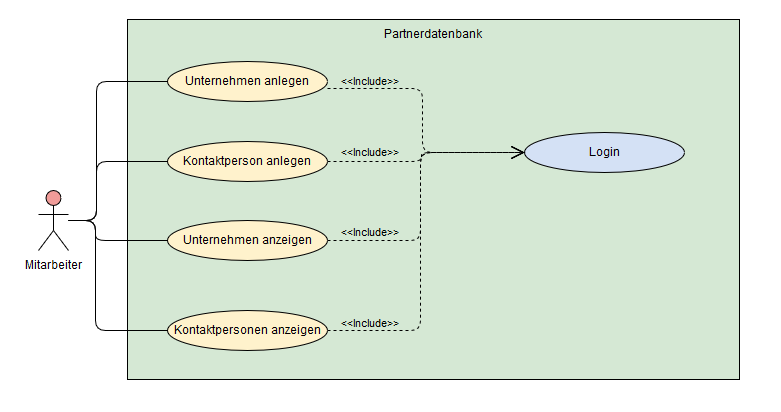
\includegraphics[scale=0.70]{Partnerdatenbank_UseCases.png}
		\caption[Anwendungsfalldiagramm der Partnerdatenbank]{Anwendungsfalldiagramm der Partnerdatenbank}
		\label{fig:UseCaseDiagramm}
	\end{center}
\end{figure}


\subsection{Lifecycle der Daten}
Weitere Geschäftsprozesse, welche die Daten der 3 Banken IT GmbH durchlaufen und in die Partnerdatenbank integriert werden, sind:
\begin{enumerate}
	\item Erstkontakt,
	\item Angebotsanfrage/Ausschreibung,
	\item Angebotslegung,
	\item Verpflichtungserklärung,
	\item Auftrag,
	\item Lieferung,
	\item Rechnung,
	\item Installation,
	\item Inbetriebnahme,
	\item Kündigung,
	\item Deaktivierung,
	\item Deinstallation.
\end{enumerate}

Diese werden jedoch nicht vom Ersteller dieser Anwendung integriert, sondern von der 3 Banken IT GmbH selbst. Diese Arbeit dient lediglich als Vorlage und Schablone für die 3 Banken IT GmbH zur Integration weiterer Services bzw. Geschäftsfälle.

\section{Beschreibung der Datenbank}
Die Datenbanken für die 3 Banken IT GmbH bestehen aus Microsoft SQL Server-Datenbanken. Ein  Microsoft SQL Server ist ein relationales Datenbankmanagementsystem (DBMS), das von Microsoft entwickelt wurde. Dieses DBMS wurde von der 3 Banken IT GmbH vorgegeben. Der Verfasser dieser Arbeit beschreibt deshalb die Charakteristiken und Vor- und Nachteile dieses DBMS nicht genauer.

\subsection{Lokale Entwicklung}
Die Datenbank wird lokal über das in Listing \ref{lst:Dockerfile.local} dargestellte Dockerfile definiert.
\begin{lstlisting}[language=docker, caption=Dockerfile für die lokale Entwicklung, label={lst:Dockerfile.local}]
	FROM mcr.microsoft.com/mssql/server:2017-latest
	EXPOSE 1433
	COPY ./create-db.sql .
	USER root
	ENV MSSQL_DEVELOPER=sa
	ENV MSSQL_SA_PASSWORD=Ruhsi@1234
	ENV ACCEPT_EULA=Y
	RUN chgrp -R 0 /var/opt && \
		chmod -R g=u /var/opt && \
		chown -R 10001:0 /var/opt && \
		( /opt/mssql/bin/sqlservr --accept-eula & ) | \
			grep -q "Service Broker manager has started" && \
		/opt/mssql-tools/bin/sqlcmd -S localhost -U \
			sa -P Ruhsi@1234 -d master -i create-db.sql
\end{lstlisting}

Im Folgenden werden die Befehle des Dockerfiles beschrieben:
\begin{enumerate}
	\item Der \textbf{FROM}-Befehl definiert das Basis Image, das bereits einen vollständigen MS SQL Server beinhaltet. Dieses Image ist in der Registry von Microsoft zu finden und kann einfach verwendet werden.
	\item Der \textbf{EXPOSE}-Befehl gibt den Port 1433 des Containers nach außen frei, sodass auch externe Clients auf dieses Service Zugriff haben.
	\item Der \textbf{COPY}-Befehl kopiert die \textit{create-db.sql}-Datei in den Container. Diese Datei muss unter dem angegebenen Pfad verfügbar sein und enthält in diesem Fall lediglich zwei Zeilen (Listing \ref{lst:create-sql}).
\begin{lstlisting}[language=sql, caption=create-db.sql, label=lst:create-sql]
	CREATE DATABASE PartnerDB;
	CREATE DATABASE DocsisDB;
\end{lstlisting}
	Zur Speicherung der Partner sowie Unternehmen ist die \textit{PartnerDB} vorgesehen. Für die Speicherung der Links der Partner zu den entsprechenden Dokumenten ist die \textit{DocsisDB} vorgesehen. Die Dokumente zu den Partnern kommen aus dem Docsis-System der 3 Banken IT GmbH. Da der Verfasser auf dieses System keinen Zugriff hat, wurde beschlossen, dass die Daten in einer eigenständigen Datenbank gemockt werden.
	\item Der \textbf{USER}-Befehl setzt den User, mit dem die darauffolgenden Befehle ausgeführt werden. In diesem Fall wird der root-User verwendet, da laut Dokumentation dieses Basis Image nur mit Root-Rechten ausgeführt werden kann.
	\item Der \textbf{ENV}-Befehl setzt Environment-Variablen. Die beiden Environment-Variablen \textit{MSSQL\_DEVELOPER} und \textit{MSSQL\_SA\_PASSWORD} setzen die Login-Parameter, mit denen auf den SQL-Service zugegriffen werden kann. Mit der Environment-Variable \textit{ACCEPT\_EULA} wird das \glqq \href{https://documentation.commvault.com/commvault/v11/article?p=50060.htm}{End-User License Agreement}\grqq akzeptiert.
	\item Im \textbf{RUN}-Befehl werden gleich mehrere Schritte ausgeführt. Die Befehle in Zeile 8, 9 und 10 setzen den Besitzer der Dateien und Unterordner des angegebenen Pfades und gewähren ihm Zugriff auf alle Dateien darin. Dadurch können die Befehle in Zeile 11 und 12 mit dem root-User ausgeführt werden.
	\item Der Befehl in Zeile 11 startet den MS SQL Server und akzeptiert das EULA. Danach wird mit dem grep-Befehl solange gewartet, bis der SQL Server hochgefahren ist und in den Logs die Ausgabe \glqq Service Broker manager has started\grqq{} zu sehen ist.
	\item In Zeile 12 verbindet sich der User mithilfe des sqlcmd-Tools und den angegebenen Parametern zum MS SQL Server und führt das oben angeführte \textit{create-db.sql}-Skript aus.
\end{enumerate}

Dieses Dockerfile kann mit folgendem Befehl gebaut werden:
\begin{lstlisting}[language=bash]
$ docker build -t docsisdb .
\end{lstlisting}
Der Parameter \textit{-t docsisdb} vergibt einen Namen für das Image. Der Punkt am Ende des Befehls ist der Pfad zum Dockerfile, in diesem Fall wird der Befehl im selben Verzeichnis wie das Dockerfile ausgeführt.

Mit dem Befehl:
\begin{lstlisting}[language=bash]
$ docker run -d -p 1434:1433 --name docsisdb docsisdb
\end{lstlisting}
wird ein Docker Container aus dem Docker Image gestartet. Die Option \textit{-d} startet den Container im Hintergrund (detached). Die Option \textit{-p 1434:1433} leitet alle Aufrufe des Ports 1434 auf den container-internen Port 1433 weiter. Auf diesem Port ist der MS SQL Server erreichbar. Mit der Option \textit{-{}-name docsisdb} wird dem Docker Container der Name \glqq docsisdb\grqq{} zugewiesen. Dadurch startet der Docker Container und der MS SQL Server ist unter dem Port 1434 des Hosts verfügbar.

Zum vereinfachten Ausführen mehrerer Docker Container ist es bei Docker auch möglich ein \textit{docker-compose.yml} zu definieren, in dem mehrere Services definiert und ausgeführt werden.
In der Datei in Listing \ref{lst:docker-compose.yml} wird das docker-compose.yml zum Ausführen der beiden Dockerfiles der docsis-database und der partner-database beschrieben:
\begin{lstlisting}[language=docker-compose-2, caption={docker-compose.yml}, label=lst:docker-compose.yml]
	version: '3'
	services:
		partner-database:
			build: ./partner-database
			container_name: "partner-database"
			ports:
				- 1433:1433
	
		docsis-database:
			build: ./docsis-database
			container_name: "docsis-database"
			ports:
				- 1434:1433
\end{lstlisting}
Im \textbf{build} wird der Pfad zu den jeweiligen Dockerfiles gesetzt. Mit \textbf{container\_name} kann der Name des Containers gesetzt werden und im \textbf{ports}-Abschnitt werden die Ports freigegeben.

Mit dem Befehl:
\begin{lstlisting}[language=bash]
	$ docker-compose up
\end{lstlisting}
werden nun beide Docker Container gestartet und sind unter den jeweiligen Ports aufrufbar.

Die beiden Docker Container können mit folgendem Befehl wieder beendet werden:
\begin{lstlisting}[language=bash]
	$ docker-compose down
\end{lstlisting}

\subsection{Deployment in OpenShift}
Das Dockerfile und die create-db.sql-Datei sehen beim Deployment der Datenbank in OpenShift gleich aus. Sie verändern sich nicht. Dadurch ist sichergestellt, dass sich die Umgebungen lokal und in OpenShift gleich verhalten. Das Deployment gestaltet sich jedoch etwas aufwändiger als lediglich ein \glqq docker run\grqq-Befehl. Da es für MS SQL Server kein vordefiniertes Template in OpenShift gibt, muss das Docker Image in die OpenShift-interne Docker Registry gepusht werden.

Folgende Schritte müssen dafür unternommen werden:
\begin{enumerate}
	\item \textbf{Freigeben der Route}: Die OpenShift-interne Docker Registry muss nach außen freigegeben werden, um diese von der CLI aus aufzurufen. Dies kann in der Web Console von OpenShift von einem Administrator erledigt werden.
	\item \textbf{Holen der Route}: Mit dem Befehl:
\begin{lstlisting}[language=bash]
	$ oc get route
\end{lstlisting}
	kann die Route der Docker Registry geholt werden.
	\item \textbf{Einloggen in die Docker Registry}: Mit dem Befehl:
\begin{lstlisting}[language=bash]
	$ docker login -u <openshift_username> -p <openshift_password> 
		<registry_route>
\end{lstlisting}
	erfolgt der Login in die die OpenShift-interne Docker Registry.
	\item \textbf{Bauen des Docker Images lokal}: Mit folgendem Befehl wird das Docker Image mit dem Namen mssql versehen und gebaut:
\begin{lstlisting}[language=bash]
	$ docker build -t mssql .
\end{lstlisting}
	\item \textbf{Taggen des Images in der Registry}: Mit dem Befehl:
\begin{lstlisting}[language=bash]
	$ docker tag mssql <registry_route>/<namespace>/mssql
\end{lstlisting}
	wird ein Tag in der OpenShift-internen Registry erstellt. Dadurch wird eine Referenz des lokalen Docker Images zum OpenShift-internen Docker Image erstellt.
	\item \textbf{Pushen des Images in die Registry}: Durch den Befehl:
\begin{lstlisting}[language=bash]
	$ docker push <registry_route>/<namespace>/mssql
\end{lstlisting}
	wird das Docker Image in die OpenShift-interne Registry gepusht.
	Dadurch kann das Docker Image in OpenShift referenziert und ausgeführt werden.
	\item \textbf{Ausführen des Image}: Mit folgendem Befehl kann das Docker Image in OpenShift gebaut werden:
\begin{lstlisting}[language=bash]
	$ oc new-app mssql
\end{lstlisting}
	Dadurch wird der Docker Container in OpenShift ausgeführt und kann intern durch die Route \textit{mssql:1433} erreicht werden. Muss die App auch von extern erreicht werden können, muss die Route vorher freigegeben werden. Dies kann einfach über die Web Console erreicht werden.
\end{enumerate}

\section{Backend-Beschreibung}
In diesem Abschnitt wird der grundsätzliche Aufbau einer Backend-Applikation beschrieben.

\subsection{Paketstruktur}
In Abbildung \ref{fig:package_structure_partner_service} ist die Paketstruktur des \textit{partner-services} zu sehen.

Im Folgenden werden die wichtigsten Pakete näher beschrieben:
\begin{itemize}
	\item \textbf{src.main}
	\begin{itemize}
		\item \textbf{fabric8}:
		\begin{itemize}
			\item  Im \textit{fabric8}-Ordner befinden sich das \textbf{deployment.yml} und das \textbf{route.yml}, die für das Deployment in OpenShift notwendig sind. Diese werden in einem späteren Abschnitt näher beschrieben.
		\end{itemize}
		\item \textbf{java.at.fh.se.master.partner}
		\begin{itemize}
			\item \textbf{aspects}: In diesem Paket befindet sich die Klasse \textit{LoggingAspect.java}, die für das Logging jeder Methode im Paket \textbf{rest} zuständig ist.
			\item \textbf{configuration}: In diesem Paket befindet sich die Klasse \textit{SimpleCORSFilter.java}. Diese setzt die Origin-Header, damit das Frontend auf die Ressourcen zugreifen kann.
			\item \textbf{rest}: Im rest-Paket befinden sich die Interfaces und Implementierungen der REST-Api. Auch die Repositories für den Zugriff auf die Datenbank und eine \textit{RestTemplateProvider}-Klasse, die das RestTemplate für REST-Aufrufe zum Docsis-Service zu Verfügung stellt, sind in diesem Paket enthalten. 
			\item \textbf{security}: In diesem Paket sind die Sicherheitskonfigurationen für den Login und die weiteren authentifizierten Aufrufe enthalten. Zudem sind Modelklassen für den User und die Rolle enthalten.
			\item \textbf{service}: In diesem Paket ist ein Service für die Interaktion mit dem Docsis-Service enthalten. Damit können alle Links von einem Partner geholt, hinzugefügt und gelöscht werden.
		\end{itemize}
		\item \textbf{resources}
		\begin{itemize}
			\item In diesem Paket ist die Datei \textit{application.yml} enthalten, die zur Konfiguration der Applikation benötigt wird. Diese wird später näher erläutert.
		\end{itemize}
	\end{itemize}
	\item \textbf{src.test}
	\begin{itemize}
		\item \textbf{java.at.fh.se.master.partner}
		\begin{itemize}
			\item \textbf{rest.controller}:
			\begin{itemize}
				\item In diesem Paket befinden sich die Tests für die Controller-Klassen.
			\end{itemize}
		\end{itemize}
	\end{itemize}
\end{itemize} 

\begin{figure}[H]
	\begin{center}
		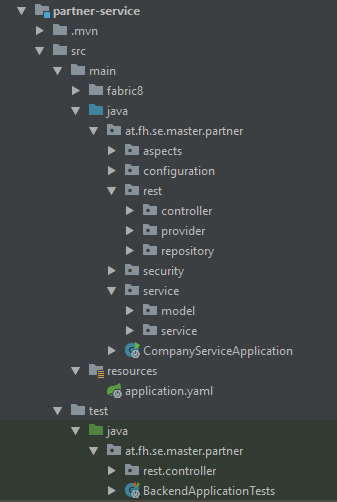
\includegraphics[scale=0.80]{package_structure_partner_service.png}
		\caption[Paketstruktur des Partnerservices]{Paketstruktur des Partnerservices}
		\label{fig:package_structure_partner_service}
	\end{center}
\end{figure}

\subsection{Logging}
Das Logging wird mithilfe von aspektorientierter Programmierung gelöst. Aspektorientierte Programmierung ist ein Paradigma, das darauf abzielt, die Modularität von Applikationen zu erhöhen. Dadurch wird zusätzliches Verhalten zum Code hinzugefügt, ohne den eigentlichen Code verändern zu müssen. Der neue Code und das zusätzliche Verhalten werden getrennt voneinander deklariert. 

In diesem Service wird aspektorientierte Programmierung zum Loggen der Ausführung von REST-Methoden genutzt. Dazu wird die Maven-Dependency in Listing \ref{lst:springbootstarteraop} benötigt.

\begin{lstlisting}[language=xml, caption=pom.xml, label=lst:springbootstarteraop]
	<dependency>
		<groupId>org.springframework.boot</groupId>
		<artifactId>spring-boot-starter-aop</artifactId>
	</dependency>
\end{lstlisting}

Die Deklaration des Aspekts sieht, wie in Listing \ref{lst:LoggingAspect} dargestellt, aus.

\begin{lstlisting}[language=java, caption={LoggingAspect.java}, label=lst:LoggingAspect]
	@Aspect
	@Component
	public class LoggingAspect {
		@Around("execution(public * at.fh.se.master.partner.rest..*(..))")
		public Object profileAllMethods(ProceedingJoinPoint proceedingJoinPoint);
	}
\end{lstlisting}

Die Klasse wird mit der Annotation \textit{@Aspect} als Aspekt gekennzeichnet. In der Klasse selbst wird ein Around-Advice deklariert. Dadurch werden alle public-Methoden mit jeglichem Rückgabeparameter im Verzeichnis \textit{at.fh.se.master.partner.rest} geloggt. Statt dem eigentlichen Aufruf der Methode wird der Aspekt aufgerufen. In diesem erfolgt das Logging. Danach muss die eigentliche Methode ausgeführt werden. Über den Parameter \textit{ProceedingJoinPoint proceedingJoinPoint} können Informationen über die Methodensignatur geholt werden. Über diesen Parameter kann auch die eigentliche Methode aufgerufen werden. Der Rückgabewert der eigentlichen Methode wird auch im Advice zurückgegeben.

\subsection{CORS-Filter}
Um einen Cross-Origin Resource Sharing (CORS)-Fehler beim Aufruf vom Frontend zu vermeiden, muss ein CORS-Filter implementiert werden. Dazu kann einfach das Interface \textit{Filter} implementiert werden. Danach muss die Methode \textit{doFilter} überschrieben werden. In dieser können die entsprechenden Header gesetzt werden.

Die Implementierung dazu zeigt Listing \ref{lst:SimpleCORSFilter}.
\begin{lstlisting}[language=java, caption={SimpleCORSFilter.java}, label=lst:SimpleCORSFilter]
	@Component
	public class SimpleCORSFilter implements Filter {
		@Override
		public void doFilter(ServletRequest req, ServletResponse resp,
		FilterChain chain) throws IOException, ServletException {
			HttpServletResponse response = (HttpServletResponse) resp;
			HttpServletRequest request = (HttpServletRequest) req;
			response.setHeader("Access-Control-Allow-Origin", request.getHeader("Origin"));
			...
		}
	}
\end{lstlisting}

Durch die beiden Parameter \textit{ServletRequest req} und \textit{ServletResponse resp} kann auf Informationen des Http-Requests und der Http-Response zugegriffen werden.
In diesem Prototyp wird der Header \textit{Access-Control-Allow-Origin} der Response mit dem Request-Header \textit{Origin} gesetzt. Dies erlaubt jeder Domain Zugriff auf diesen Server. Dies muss von der 3 Banken IT GmbH natürlich auf die entsprechende Domäne, in der das Frontend in der Produktivumgebung läuft, geändert werden.

\subsection{Controller}
Mit Controllern kann eine REST-Api bereitgestellt werden. Mit \textit{@RequestMapping} wird der grundsätzliche Pfad zu diesem Controller gesetzt. Die Annotation \textit{@CrossOrigin} ist ein Mechanismus, der von Spring Boot bereitgestellt wird und beim Handling von CORS unterstützt. Diese Annotation kann auch auf Klassenebene verwendet werden.
Durch die Annotation \textit{@PostMapping} wird die Methode als POST-Aufruf definiert. Diese ist in diesem Beispiel unter dem Pfad \glqq company\grqq{} verfügbar. Der Body des Requests muss in der Form von JSON vorliegen und diese Methode liefert auch Responsedaten in Form von JSON zurück. Die beiden Annotationen \textit{@ResponseBody} und \textit{@RequestBody} mappen den Rückgabewert bzw. den Inputparameter zu JSON. 
Der Inputparameter darf aufgrund der Annotation \textit{@NotNull} nicht null sein. Dieser muss auch durch die \textit{@Valid}-Annotation valide sein. In der Klasse Company können für einzelne Member Beschränkungen angegeben werden. Diese werden durch die Annotation @Valid validiert. Ein Beispiel für einen Controller zeigt Listing \ref{lst:CompanyControllerApi}.

\begin{lstlisting}[language=java, caption=CompanyControllerApi.java, label=lst:CompanyControllerApi]
	@RequestMapping("/")
	public interface CompanyControllerApi {
		...
	
		@CrossOrigin
		@PostMapping(value = "company",
			produces = MediaType.APPLICATION_JSON_VALUE,
			consumes = MediaType.APPLICATION_JSON_VALUE)
		@ResponseBody
		ResponseEntity<Company> addCompany(@RequestBody @NotNull 
			@Valid Company company);
		
		...
	}
\end{lstlisting}

\subsection{Sicherheitskonfiguration}
Durch Erweitern der Klasse \textit{WebSecurityConfigurerAdapter} kann die Sicherheitskonfiguration für Spring Boot-Applikationen einfach definiert werden.
Dadurch muss die Methode \textit{configure} überschrieben werden. Diese liefert die Klasse \textit{HttpSecurity}, mit der die Konfiguration vorgenommen werden kann. Listing \ref{lst:SecurityConfiguration} zeigt die Sicherheitskonfiguration für das Partner-Service.  

\begin{lstlisting}[language=java, caption={SecurityConfiguration.java}, label=lst:SecurityConfiguration]
	@Configuration
	public class SecurityConfiguration extends WebSecurityConfigurerAdapter {
		@Override
		protected void configure(HttpSecurity http) throws Exception {
			http
				.cors().configurationSource(corsConfigurationSource()).and()
				.authorizeRequests()
				.antMatchers("/login").permitAll()
				.antMatchers("/actuator/health").permitAll()
				.anyRequest().authenticated()
				.and()
				.formLogin()
				.loginProcessingUrl("/login")
				.usernameParameter("username")
				.passwordParameter("password")
				.successHandler(this::loginSuccessHandler)
				.failureHandler(this::loginFailureHandler)
				.and()
				.logout()
				.logoutUrl("/logout") 
				.logoutSuccessHandler(this::logoutSuccessHandler)
				.invalidateHttpSession(true).and()
				.exceptionHandling()
				.authenticationEntryPoint((httpServletRequest, httpServletResponse, e) ->
					httpServletResponse.setStatus(HttpStatus.UNAUTHORIZED.value()));
		}
	}
\end{lstlisting}

Im Folgenden werden die einzelnen Konfigurationseinstellungen beschrieben:
\begin{itemize}
	\item \textbf{cors} und \textbf{configurationSource}: Mit diesen beiden Parametern können weitere Einstellungen bezüglich CORS vorgenommen werden.
	\item \textbf{authorizeRequests}: Mit dieser Einstellung können jegliche REST-Aufrufe nur autorisiert aufgerufen werden.
	\item \textbf{antMatchers}: Durch diese beiden Einstellungen können Ausnahmen für die Autorisierung definiert werden. Diese sind nötig für den Login-Aufruf und den Health-Check.
	\item \textbf{formLogin}: In den Zeilen 12 bis 17 im Listing \ref{SecurityConfiguration} wird der Login als Form-Login unter der URL \textit{login} mit den Parametern \glqq username\grqq{} und \glqq password\grqq{} definiert. Zusätzlich wird ein \textit{successHandler} und \textit{failureHandler} für den erfolgreichen bzw. fehlerhaften Login definiert.
	\item \textbf{logout}: Auch für den Logout wird eine URL und ein \textit{successHandler} definiert.
	\item \textbf{exceptionHandling}: In den Zeilen 23 und 24 wird eine Default-Nachricht bei unautorisierten Aufrufen definiert.
\end{itemize}

\subsection{Docsis-Service}
Im Unterpaket \textit{service} befindet sich die Klasse \textbf{DocsisService}. Diese dient zum Managen der Links im Docsis-Service. Da das Docsis-Service ein eigenständiges Microservice ist, werden dazu REST-Aufrufe benötigt. Spring Boot stellt dabei die Klasse RestTemplate zur Verfügung. Damit können die REST-Aufrufe einfach wie in Listing \ref{lst:DocsisService.java} erledigt werden:

\begin{lstlisting}[language=java, caption={DocsisService.java}, label={lst:DocsisService.java}]
	@Component
	public class DocsisService {
	
		private final RestTemplate restTemplate;
		
		@Value(value = "${base.service.docsis}")
		private String restBaseServiceDocsis;
		
		@Autowired
		public DocsisService(RestTemplate restTemplate) {
			this.restTemplate = restTemplate;
		}
		
		public ResponseEntity<List<Link>> getAllLinksOfPartner(Long partnerId) {
			List<Link> links = restTemplate.getForObject(restBaseServiceDocsis +
				"links/partner/" + partnerId, ArrayList.class);
			return new ResponseEntity<>(links, HttpStatus.OK);
		}
	}
\end{lstlisting}

Das RestTemplate wird dabei über Konstruktorinjektion injiziert. Die URL zum Docsis-Service befindet sich als Konfigurationsparameter im application.yml und wird über die Annotation @Value geladen.
Mit der Methode \textit{getForObject} des RestTemplate-Objektes kann ein GET-Aufruf zur angegeben URL gemacht werden. Der Parameter \textit{ArrayList.class} gibt an, dass der Body der Response vom Typ \textit{ArrayList} ist.
Das Speichern eines Links und Löschen eines Links sehen sehr ähnlich aus und können auch mit dem RestTemplate einfach implementiert werden.


\subsection{application.yml}
Die \textbf{applicationy.yml}-Datei dient zur Konfiguration der Anwendung und ist in verschiedene Profile aufgeteilt. Dadurch kann lokal eine andere Datenbankverbindung als in OpenShift verwendet werden. In Listing \ref{application.yml.dev} wird das Profil \textit{dev} näher beschrieben:

\begin{lstlisting}[language=yml, caption={application.yml}, label={application.yml.dev}]
	spring:
		profiles: dev
		datasource:
			url: jdbc:sqlserver://127.0.0.1:1433;databaseName=PartnerDB
			username: <username>
			password: <password>
	base:
		service:
			docsis: http://localhost:8080/
	server:
		port: 8090
	opentracing:
		jaeger:
			udp-sender:
				host: localhost
				port: 6831
\end{lstlisting}

Das Profil \textit{dev} wird für die Entwicklung lokal verwendet. Bei der Konfiguration der Datenbank müssen zumindest die \textit{url}, der \textit{username} und das \textit{password} angegeben werden. Der Parameter \textit{base.service.docsis} dient zum Erreichen des Docsis-Services. Dadurch kann auch auf verschiedenen Umgebungen der REST-Endpoint des Docsis-Services einfach konfiguriert werden. Dieser wird in Listing \ref{lst:DocsisService.java} mit der Annotation \textit{@Value} verwendet.
Der Parameter \textit{server.port} dient zur Spezifikation des Ports, hinter dem die Applikation läuft. Dieser ist standardmäßig 8080. Da das Docsis-Service auf Port 8080 konfiguriert ist, muss das Partner-Service auf einem anderen Port laufen, um Kollisionen zu vermeiden.
Die \textit{opentracing}-Parameter dienen zur Konfiguration von Jaeger. Diese werden in Abschnitt \ref{sec:tracingwithjaeger} weiter beschrieben.

\section{Frontend-Beschreibung}
Das Frontend ist eine Angular 8-Applikation und dient zur erleichterten Durchführung der Geschäftsfälle. Auch der rollenbasierte Login ist im Frontend implementiert. Grundsätzlich kann jeder Mitarbeiter jede Aktion durchführen. Dies soll in Zukunft, sobald weitere Geschäftsfälle integriert werden, eingeschränkt werden. 

Loggt sich ein User ein, sieht er alle Unternehmen und Partner der 3 Banken IT GmbH. Durch eine eingebaute Navigation können weitere Reiter, wie Partner anlegen oder Unternehmen anlegen, aufgerufen werden. Im Header der Anwendung kann sich der User wieder ausloggen und gelangt dadurch zum Login zurück. Nur eingeloggte User können Aktionen durchführen.

\subsection{Paketstruktur}
In Abbildung \ref{fig:package_structure_frontend} ist die Paketstruktur vom \textit{Frontend} zu sehen.

Im Folgenden werden die wichtigsten Verzeichnisse genauer beschrieben:
\begin{itemize}
	\item \textbf{src.main.angular.src}
	\begin{itemize}
		\item \textbf{app}: Im app-Verzeichnis befindet sich die eigentliche Anwendung. Diese besteht aus den folgenden Verzeichnissen:
		\begin{itemize}
			\item \textbf{main-pages}: Mit dem Frontend können die Geschäftsfälle \textit{Unternehmen anlegen}, \textit{Parnter anlegen}, \textit{Partner anzeigen}, \textit{Unternehmen anzeigen} abgewickelt werden. Im Verzeichnis main-pages befinden sich die Komponenten für die jeweiligen Geschäftsfälle.
			\item \textbf{models}: In diesem Verzeichnis befinden sich die Modelklassen für den User, ein Unternehmen, einen Partner und einen Link.
			\item \textbf{services}: Im Verzeichnis services befinden sich die Angular-Services zur Durchführung der REST-Calls für die einzelnen Geschäftsfälle.
			\item \textbf{shared}: Im Verzeichnis shared befinden sich viele unterschiedliche Komponenten, die für die Anwendung nötig sind. Dazu gehören Guards zur Absicherung der Routen, Interceptors, wie z.B. der HTTP-Interceptor zum Setzten von Header und Komponenten zur Darstellung der Navigation und des Headers.
 			\item \textbf{signin}: Das Verzeichnis signin besteht aus einer Login-Komponente und einem Authentifizierungsservice.
		\end{itemize}
		\item \textbf{configuration}: Im Verzeichnis configuration befindet sich die Konfiguration der einzelnen Unterseiten sowie ein HTTP-Header Objekt zur Verwendung im Interceptor. Diese Konfiguration ist bei allen environments gleich.
		\item \textbf{environments}: In diesem Verzeichnis befindet sich die Konfiguration der Backend-URL. Diese ist environment-spezifisch und kann daher nicht im configuration-Verzeichnis gewartet werden.
	\end{itemize}
\end{itemize}


\begin{figure}[H]
	\begin{center}
		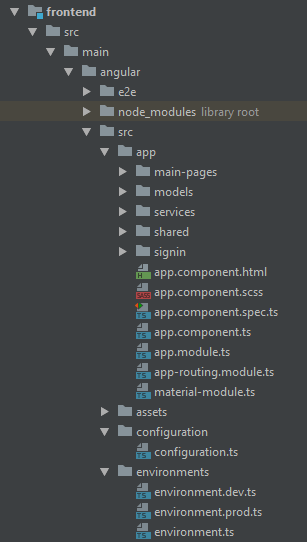
\includegraphics[scale=0.70]{package_structure_frontend.png}
		\caption[Paketstruktur des Frontends]{Paketstruktur des Frontends}
		\label{fig:package_structure_frontend}
	\end{center}
\end{figure}

\subsection{Environment-Konfiguration}
Die Konfiguration der Environments gestaltet sich sehr einfach. Durch das Hinzufügen eines Codesnippets Listing \ref{lst:angular.json} in die \textit{angular.json}-Datei wird beim Starten der Anwendung mit dem Parameter \textit{-{}-configuration=<environment>} die Datei \textit{environment.ts} mit der Datei environment.<environment>.ts ausgetauscht. Z.B. beim Start der Anwendung mit dem Befehl:
\begin{lstlisting}[language=bash]
$	ng serve --configuration=dev
\end{lstlisting}
 
wird anstatt der Datei environment.ts die Datei environment.dev.ts verwendet. In dieser Datei sind die URL´s zum Backend beim Deployment in OpenShift konfiguriert.

\begin{lstlisting}[language=json, caption={angular.json}, label={lst:angular.json}]
	...
	"configurations": {
		"dev": {
			"fileReplacements": [
			{
				"replace": "src/environments/environment.ts",
				"with": "src/environments/environment.dev.ts"
			}
		]
	},
	...
\end{lstlisting}

\subsection{Konfiguration}
In der configuration.ts-Datei sind die einzelnen Seiten und ein HTTP-Header definiert.

\begin{lstlisting}[language=JavaScript, caption={configuration.ts}, label={lst:configuration.ts}]
	export const configuration = {
		...
		PAGES: {
			HOME: '/home',
			ADDPARTNER: '/addpartner',
			PARTNER: '/partner',
			ADDCOMPANY: '/addcompany',
			COMPANY: '/company',
			LOGIN: '/login'
		},
		...
	}
\end{lstlisting}
Auf den Parameter \textit{HOME} im Listing \ref{lst:configuration.ts} kann im TypeScript-Code mittels \textit{configuration.PAGES.HOME} zugegriffen werden.

\subsection{Anwendung}
In der Anwendung können die Geschäftsfälle \textit{Unternehmen hinzufügen}, \textit{Unternehmen löschen}, \textit{Unternehmen anzeigen} und \textit{Partner anzeigen} abgewickelt werden. Die Logik für diese Geschäftsfälle ist im Verzeichnis \textit{main-pages} enthalten.
Je nach derzeitiger URL wird auf die richtige Komponente geroutet. Die Routing-Regeln sind in der Datei \textit{app-routing.module.ts} definiert. Ein Ausschnitt dieser Datei wird in Listing \ref{lst:app-routing.module.ts} gezeigt.

\begin{lstlisting}[language=JavaScript, caption={app-routing.module.ts}, label={lst:app-routing.module.ts}]
	export const routes: Routes = [
		...
		{
			path: 'home',
			component: MainLayoutComponent,
			loadChildren: () => HomePagesModule,
			data: {pageTitle: 'Home'},
			canActivate: [UserAuthenticationGuard]
		},
		...
\end{lstlisting}
Diese Komponente ist unter dem Pfad \glqq /home\grqq{} erreichbar Die Komponente \textit{MainLayoutComponent} wird dadurch inklusive dem Kindmodul \textit{HomePagesModule} gerendert. Der Header und die Navigation sind in der MainLayoutComponent definiert. Diese lädt danach die HomePagesModule hinzu, in der die eigentliche Logik stattfindet. Durch den \textit{UserAuthenticationGuard} wird überprüft, ob der eingeloggte User diese Seite aufrufen darf.

Für die REST-Aufrufe werden Services verwendet. In diesen wird der HttpClient von Angular injiziert. Dadurch können einfach verschiedene REST-Methoden ausgeführt werden.
Listing \ref{lst:partner.service.ts} zeigt einen Ausschnitt der Datei \textit{partner.service.ts}:

\begin{lstlisting}[language=JavaScript, caption={partner.service.ts}, label={lst:partner.service.ts}]
	export class PartnerService {
		...
		private readonly URL = environment.backendOriginSegment + ":" +
			environment.backendOriginPort;
		
		constructor(private http: HttpClient) {}
	
		addOrUpdatePartner(id: number, partner: Partner): Observable<Partner> {
			return this.http.post<Partner>(this.URL + "/company/" + id + "/partner",
				JSON.stringify(partner, partner.constructor.prototype),
					.pipe(
						retry(1)
					);
		}
		...
	}
\end{lstlisting}
Durch die environment-Datei wird die URL aus Host und Port zusammengebaut. Dadurch wird sichergestellt, dass lokal und in OpenShift die richtige URL für das Backend verwendet wird, ohne Code ändern zu müssen.

Beim Aufruf der Methode \textit{addOrUpdatePartner} wird ein POST-Aufruf zur entsprechenden URL mit dem Objekt \textit{Partner} im Body durchgeführt. Die retry-Pipe gibt an, wie oft dieser Aufruf bei einem Fehlversuch wiederholt werden soll. Diese Methode gibt ein Observable zurück, auf das registriert werden kann. 

Der Aufruf dieser Methode sieht, wie in Listing \ref{lst:addPartner} gezeigt, aus.
\begin{lstlisting}[language=JavaScript, caption={addPartner-Methode}, label={lst:addPartner}]
	addPartner(): void {
		this.addOrUpdatePartnerSubscription = 
			this.partnerService.addOrUpdatePartner(this.selectedCompany.id, this.partner)
				.subscribe((partner: Partner) => {
					...
				})
	}
\end{lstlisting}

Die \textit{addOrUpdatePartner}-Methode im PartnerService wird mittels der UnternehmensID und dem veränderten oder neu hinzugefügten Partner aufgerufen. Dadurch, dass diese Methode ein Observable zurückliefert, kann man sich mittels der Methode \textit{subscribe} auf dieses Observable registrieren. Sobald die Response vom Server kommt, wird der Code in der \textit{subscribe}-Methode aufgerufen.

\subsection{Starten der Anwendung}
\textbf{Lokal} kann das Frontend über folgenden Kommandozeilenbefehl gestartet werden:
\begin{lstlisting}[language=bash]
$ ng serve --configuration=dev
\end{lstlisting}

Mittels dem Parameter \textit{-{}-configuration=dev} wird das lokale Environment gestartet. Mittels \textit{ng serve} wird ein von Angular mitgelieferter Webserver hochgefahren. In diesem läuft die Applikation und kann im Browser unter der URL \textit{http://localhost:4200} aufgerufen werden.

Mit folgendem Befehl kann die Applikation in \textbf{OpenShift} deployt werden:
\begin{lstlisting}[language=bash]
$ npx nodeshift --dockerImage=nodeshift/ubi8-s2i-web-app 
	--imageTag=10.x --build.env OUTPUT_DIR=dist/frontend --expose
\end{lstlisting}

Nodeshift ist ein Kommandozeilentool zum Deployment von Node.js-Anwendungen in OpenShift. Dabei wird das Docker Image \textit{nodeshift/ubi8-s2i-web-app} mit dem Image Tag \textit{10.x} verwendet. 
Das Output-Directory wird auf \textit{dist/frontend} gesetzt. Dies ist das Verzeichnis, in dem die Applikation gebaut wird. Mittels \textit{-{}-expose} wird die Route der Applikation in OpenShift freigegeben und ist damit durch einen Browser erreichbar.
\chapter{Design und Implementierung der Partnerdatenbank}
Im Folgenden werden das Design und die Implementierung der Partnerdatenbank und die verwendeten Technologien sowie deren Implementierung beschrieben.

\section{Microservice-Architektur}
Die gesamte Applikation wird, wie in Abbildung \ref{fig:DesignOfMicroserviceArchitecture} zu sehen, als Microservice-Architektur designt. Dabei wird die Designvariante \textit{Service-Orchestrierung} gewählt. Das Partner-Service fungiert dabei als Kompositionsservice. Das Partner-Service wird dabei zur zentralen Autorität. Dies ist jedoch auch die Schwachstelle einer Microservice-Anwendung. Fällt dieses Service aus, steht die gesamte Anwendung still. Dadurch wird das Partner-Service zum \textit{Single-Point-of-Failure} in dieser Architektur. Durch das Replizieren, Skalieren und Clustering dieses Services in OpenShift kann dieses Problem einfach gelöst werden.

Wird am Frontend ein Partner- oder Unternehmens-Objekt benötigt, ruft das Frontend das Partner-Service auf. Dieses holt sich aus der PartnerDB das entsprechende Objekt und liefert dieses als Response zurück.
Werden auch die Links zu den verschiedenen Partnern benötigt, leitet das Partner-Service den Aufruf zum Docsis-Service weiter. Dieses holt sich die entsprechenden Links zum jeweiligen Partner aus der DocsisDB und liefert diese an das Partner-Service zurück. Das Partner-Service verpackt die Links in ein Partner-Objekt und liefert das Partner-Objekt an das Frontend zurück.

Werden weitere Services hinzugefügt, ruft das Partner-Service auch diese auf und liefert die Response an das Frontend zurück. In Abbildung \ref{fig:DesignOfMicroserviceArchitecture} ist zu sehen, wie das Angebotslegungs-Service in die Applikation integriert werden kann. Dieses verwaltet die Angebote in der AngebotsDB. Da die Dokumente der Angebotslegung wahrscheinlich auch in der DocsisDB gespeichert sind, könnte das Angebotslegungs-Service auch das Docsis-Service aufrufen. Um die Struktur der Anwendung so einfach wie möglich zu halten, kann auch der Umweg über das Partner-Service erfolgen. Somit redet jedes Service lediglich mit dem Partner-Service und es ist ein klarer Workflow ersichtlich.

In OpenShift wird dann lediglich die Route des Partner-Services freigegeben. Alle anderen Services kommunizieren nur intern und sind auch nur innerhalb des Clusters aufrufbar. Dadurch ist auch der Login und die Authentifizierung sowie die Autorisierung lediglich für das Partner-Service zu implementieren, da externe Clients nur Zugriff auf dieses Service haben und alle Geschäftsfälle zuerst über das Partner-Service abgewickelt werden.

\begin{figure}[H]
	\begin{center}
		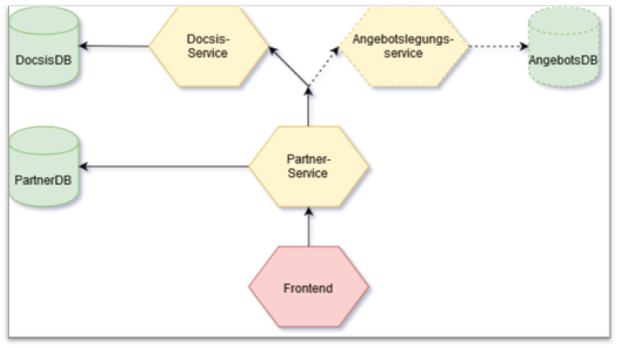
\includegraphics[scale=0.90]{DesignInOpenShift.png}
		\caption[Design der Microservice-Architektur]{Design der Microservice-Architektur}
		\label{fig:DesignOfMicroserviceArchitecture}
	\end{center}
\end{figure}

\section{Spring Boot}
Spring Boot unterstützt Entwickler bei der Erstellung von Microservice-Technologien ungemein. Spring Boot bietet dabei eine Fülle an Abhängigkeiten, die besonders für die Entwicklung von Microservices geeignet sind.

\subsection{Fehlerbehandlung mit Spring Retry}
Spring Retry bietet die Möglichkeit eine fehlgeschlagene Operation erneut ausführen zu lassen. Dies ist besonders bei REST-Aufrufen sehr wichtig. Dabei können Fehler einfacher und schneller auftreten, als wenn eine Methode eine andere Methode in derselben JVM aufgerufen werden würde. Spring Retry bietet dabei die Kontrolle über den Prozess und lässt sich einfach erweitern und anpassen \cite{SpringBootOnline}.

Bei der Verwendung von Spring Retry wird die Maven-Dependency in Listing \ref{lst:spring-retry} benötigt.
\begin{lstlisting}[language=xml, caption=pom.xml, label=lst:spring-retry]
	<dependency>
		<groupId>org.springframework.retry</groupId>
		<artifactId>spring-retry</artifactId>
	</dependency>
\end{lstlisting}

Zur Verwendung von Spring Retry muss eine Konfigurationsklasse mit \textit{@EnableRety} annotiert werden.

\subsubsection{Annotation @Retryable}
\label{ann:retryable}
\begin{lstlisting}[language=java, caption=DocsisService.java, label={lst:docsisService.retry}]
	@Retryable(value = {RestClientException.class, WebApplicationException.class},
		maxAttempts = 5,
		backoff = @Backoff(delay = 2000)
	)
	public ResponseEntity<List<Link>> getAllLinksOfPartner(Long partnerId) {
		List<Link> links = restTemplate.getForObject(restBaseServiceDocsis + 
			"links/partner/" + partnerId, ArrayList.class);
		return new ResponseEntity<>(links, HttpStatus.OK);
	}	
\end{lstlisting}

Durch den Parameter \textit{value = \{RestClientException.class, WebApplicationException.class\}} wird der Retry nur ausgeführt, wenn der Fehler vom Typ RestClientException oder WebApplicationException ist. Bei anderen Exceptions wird der Retry-Mechanismus nicht ausgelöst. 

Durch \textit{maxAttempts} kann die maximale Anzahl an Retry-Versuchen angegeben werden. Diese Methode wird bei auftretenden RestClientExceptions oder WebApplicationExceptions im Beispiel in Listing \ref{lst:docsisService.retry} maximal fünf Mal wiederholt.

Damit die Methode nicht sofort nach einem Fehlversuch neu ausgeführt wird, kann ein \textit{Backoff} angegeben werden. In diesem Fall wird zwei Sekunden nach dem Fehlversuch die Methode neu ausgeführt. \newline


\subsubsection{@Recover}
\label{ann:recover}
Eine weitere nützliche Annotation von Spring Retry ist \textit{@Recover}. Schlägt die Methode aus Listing \ref{lst:docsisService.retry} zum fünften Mal fehl, wird die Methode aus Listing \ref{lst:docsisService.recover} aufgerufen. Da sich die Behandlung bei unterschiedlichen Exceptions natürlich unterscheidet, kann die Recover-Methode auch für jede Exception explizit definiert werden. Es wird dabei automatisch die richtige Methode, die zum Typ der geworfenen Exception passt, aufgerufen.

\begin{lstlisting}[language=java, caption=DocsisService.java, label={lst:docsisService.recover}]
	@Recover
	public void recoverRestClientException(RestClientException ex){
		...
	}
	
	@Recover
	public void recoverWebApplicationException(WebApplicationException ex){
		...
	}
\end{lstlisting}

\subsubsection{Template RetryTemplate}
Spring Retry bietet auch ein Template zur generellen Konfiguration von Retry-Methoden. Im Listing \ref{lst:retryTemplate} wird eine mögliche Konfiguration von Spring Retry gezeigt.

\begin{lstlisting}[language=java, caption=RetryConfig.java, label=lst:retryTemplate]
	@Configuration
	public class RetryConfig {
		...
		@Bean
		public RetryTemplate retryTemplate() {
			RetryTemplate retryTemplate = new RetryTemplate();
			
			FixedBackOffPolicy fixedBackOffPolicy = new FixedBackOffPolicy();
			fixedBackOffPolicy.setBackOffPeriod(2000l);
			retryTemplate.setBackOffPolicy(fixedBackOffPolicy);
			
			SimpleRetryPolicy retryPolicy = new SimpleRetryPolicy();
			retryPolicy.setMaxAttempts(2);
			retryTemplate.setRetryPolicy(retryPolicy);
			
			return retryTemplate;
		}
		...
	}
\end{lstlisting}
Die \textit{RetryPolicy} bestimmt, wann oder wie oft eine Methode wiederholt werden soll. In diesem Fall zwei Mal. Die \textit{BackOffPolicy} wird zur Definition des Backoffs verwendet.

\begin{lstlisting}[language=java, caption=RetryOperations, label=lst:retryOperations]
	public interface RetryOperations {
		<T> T execute(RetryCallback<T> retryCallback) throws Exception;
		...
	}
\end{lstlisting}


Das \textit{RetryTemplate} ist eine Klasse, die das Interface RetryOperations aus Listing \ref{lst:retryOperations} implementiert. Dadurch kann das Template, wie in Listing \ref{anonymousfunction} gezeigt, aufgerufen werden.

\begin{lstlisting}[language=java, caption=Aufruf mit anonymer Funktion, label=anonymousfunction]
	retryTemplate.execute(new RetryCallback<Void, RuntimeException>() {
		@Override
		public Void doWithRetry(RetryContext arg0) {
			myService.templateRetryService();
			...
		}
	});
\end{lstlisting}

Alle Methoden innerhalb der \textit{doWithRetry}-Methode unterliegen nun der Spezifikation von RetryConfig.
Der Aufruf kann natürlich auch einfacher mit einer Lambda-Expression statt einer anonymen Funktion erfolgen (Listing \ref{lst:lambda}).

\begin{lstlisting}[language=java, caption=Aufruf mittels Lambda-Expression, label=lst:lambda]
	retryTemplate.execute(arg0 -> {
		myService.templateRetryService();
		...
	});
\end{lstlisting}


\subsection{REST-Schnittstellenbeschreibung mit Swagger}
Gerade bei Microservice-Applikationen ist es essenziell, passende Spezifikationen und Dokumentationen für die REST-Schnittstellen zu erstellen. Diese Dokumentationen sollten informativ, lesbar und einfach zu folgen sein. 

Wird diese Dokumentation manuell erstellt, werden oft Änderungen in der API nicht sofort in der Dokumentation nachgezogen. Dies ist natürlich für Aufrufer der API und Anwender des Services fatal, da Aufrufe plötzlich nicht mehr funktionieren und es scheinbar keine Änderungen gab.

Dieses Problem löst Swagger. Swagger ist ein Tool zur automatischen Dokumentation der REST-API. Dadurch ist die Dokumentation stets aktuell.

In der Partnerdatenbank wird die Springfox Implementierung von Swagger verwendet. Dazu wird die Maven-Dependency in Listing \ref{lst:springfox-swagger} benötigt.
\begin{lstlisting}[language=xml, caption=pom.xml, label=lst:springfox-swagger]
	<dependency>
		<groupId>io.springfox</groupId>
		<artifactId>springfox-swagger2</artifactId>
	</dependency>
\end{lstlisting}


Swagger wird durch die Annotation \textit{@EnableSwagger2} aktiviert. Das Docket-Bean muss definiert werden. Die \textit{select}-Methode des Docket-Beans liefert eine Instanz der Klasse \textit{ApiSelectorBuilder} zurück. Diese bietet einen Weg, um die Endpoints von Swagger zu kontrollieren. Durch die \textit{RequestHandlerSelections} wird angegeben, dass lediglich REST-Methoden im Basispaket \glqq at.fh.se.master.company\grqq{} durch Swagger dokumentiert werden.
\begin{lstlisting}[language=java, caption=Swagger-Konfiguration, label=lst:swaggerconf]
	@SpringBootApplication
	@EnableSwagger2
	public class CompanyServiceApplication {
		...
		@Bean
		public Docket productApi() {
			return new Docket(DocumentationType.SWAGGER_2)
			.select()
			.apis(
				RequestHandlerSelectors
					.basePackage("at.fh.se.master.company")
			).build();
		}
		...
	}
\end{lstlisting}

Die Swagger-Dokumentation ist nach dem Start der Applikation unter dem Link \textit{http://localhost:8080/spring-security-rest/api/v2/api-docs} erreichbar. Dies ist ein JSON-Objekt mit Key-Value Paaren. Diese Datei ist leider für Menschen nicht gut lesbar.
Springfox bietet daher mit der Maven-Dependency aus Listing \ref{lst:springfoxswaggerui} eine UI zur besseren Darstellung der REST-Methoden:

\begin{lstlisting}[language=xml, caption=pom.xml, label=lst:springfoxswaggerui]
	<dependency>
		<groupId>io.springfox</groupId>
		<artifactId>springfox-swagger-ui</artifactId>
	</dependency>
\end{lstlisting}

Die UI ist nach dem Starten der Applikation unter \textit{http://localhost:8080/swagger-ui.html} erreichbar. Sie zeigt alle REST-Methoden der Applikation in einer grafischen Darstellung. Mit dieser UI können die einzelnen REST-Methoden auch aufgerufen und getestet werden.

\subsection{Tracing mit Jaeger}
\label{sec:tracingwithjaeger}
Jaeger ist eine Applikation zum Tracen von Serviceaufrufen in Anwendungen. Bei der Implementierung einer Microservice-Architektur treten viele Probleme und Hürden auf. Diese Probleme betreffen hauptsächlich die beiden Gebiete \textbf{Netzwerke} und \textbf{Aufspürbarkeit von Services}. Es ist sehr viel komplexer, ein System bestehend aus kleinen Untersystemen zu debuggen als eine einzelne Applikation \cite{jaeger}.

Jaeger addressiert dabei folgende Probleme \cite{jaeger}:
\begin{itemize}
	\item Verteiltes Monitoring von Transaktionen.
	\item Performanz- und Latenzoptimierungen.
	\item Ursachenanalyse.
	\item Analyse der Serviceabhängigkeiten.
	\item Verteilte Propagierung von Kontexten.
\end{itemize}

Folgenden Features bietet Jaeger, um die Nutzung noch einfacher zu machen \cite{jaeger}:
\begin{itemize}
	\item \textbf{Hohe Skalierbarkeit}: Das Jaeger-Backend besitzt keinen Single-Point-of-Failure und skaliert mit den Businessanforderungen. Dies ist gerade bei der Entwicklung von Microservices von großer Bedeutung.
	\item \textbf{Nativer Support für OpenTracing}: Das Jaeger Backend, die Web UI und die Bibliotheken von Jaeger sind so designt, dass sie von Grund auf den OpenTracing-Standard unterstützen. Dazu gehören:
	\begin{itemize}
		\item das repräsentieren der Traces als direkte azyklische Graphen über Span-Referenzen,
		\item der Support von typisierten Span Tags und strukturierten Logs,
		\item der Support von verteilter Kontextpropagierung.
	\end{itemize}
	\item \textbf{Mehrere Speicher-Backends}: Jaeger unterstützt zwei populäre OpenSource NoSQL-Datenbanken als Speicher-Backends: Cassandra und Elasticsearch. Jaeger enthält auch einen In-Memory-Speicher für Test-Setups.
	\item \textbf{Modernes Web UI}: Die Jaeger Web UI wurde mit JavaScript und React entwickelt. Verschiedene Performanzverbesserungen wurden im Laufe der Jahre eingebaut, um tausende Spans zu tracen.
	\item \textbf{Cloud-Native Deployment}: Das Jaeger Backend besteht aus einer Sammlung von Docker-Containern. Das Deployment zum Kubernetes-Cluster wird durch \textit{Kubernetes Operators}, \textit{Kubernetes Templates} und \textit{Helm Charts} vereinfacht.
	\item \textbf{Beobachtbarkeit}: Alle Jaeger-Backend-Komponenten bieten standardmäßig Metriken an. Logs werden dabei mittels strukturiertem Logging auf der Konsole ausgegeben.
	\item \textbf{Rückwärtskompatibilität mit Zipkin}: Sofern bestehende Anwendungen Bibliotheken von Zipkin Web-Versionen verwenden, sind diese auch mit Jaeger kompatibel. Anwendungen, die bereits mit Zipkin getraced werden, müssen daher nicht neu geschrieben werden.
\end{itemize}

Auch für Jaeger gibt es eine UI zur Darstellung der Serviceaufrufe. Um die \textit{JaegerUI}, den \textit{collector}, die \textit{query} und den \textit{agent} inklusive einer Speicherkomponente zu starten, kann folgender Docker-Befehl in der Kommandozeile ausgeführt werden:

\begin{lstlisting}
$ docker run -d --name jaeger \
	-e COLLECTOR_ZIPKIN_HTTP_PORT=9411 \
	-p 5775:5775/udp \
	-p 6831:6831/udp \
	-p 6832:6832/udp \
	-p 5778:5778 \
	-p 16686:16686 \
	-p 14268:14268 \
	-p 14250:14250 \
	-p 9411:9411 \
	jaegertracing/all-in-one:1.17
\end{lstlisting}
Dieser Befehl startet einen Docker Container aus dem Docker Image \textit{jaegertracing/all-in-one:1.17} und gibt die entsprechenden Ports frei. Diese Applikation kann nun unter der URL \textit{http://localhost:16686} aufgerufen werden und kann Traces über die entsprechenden Ports entgegennehmen.

Für die Verwendung von Jaeger in einer Spring Boot-Applikation muss die Maven-Dependency aus Listing \ref{opentracing-spring-jaeger} hinzugefügt werden.
\begin{lstlisting}[language=xml, caption=pom.xml, label=opentracing-spring-jaeger]
	<dependency>
		<groupId>io.opentracing.contrib</groupId>
		<artifactId>opentracing-spring-jaeger-cloud-starter</artifactId>
	</dependency>
\end{lstlisting}


\begin{lstlisting}[language=yml, caption=application.yml, label=lst:jaeger.params]
	spring:
		application:
			name: partner-service
	opentracing:
		jaeger:
			udp-sender:
				host: localhost
				port: 6831
\end{lstlisting}

Um die JaegerUI lokal erreichen zu können, müssen im \textit{application.yml} zumindest die in Listing \ref{lst:jaeger.params} gezeigten Parameter angegeben werden. Die Traces dieser Applikation werden nun unter dem Namen \glqq partner-service\grqq{} angezeigt.
Der \textit{host}- und der \textit{port}-Parameter geben den Endpoint der Jaeger-CLI, hinter der der Collector sitzt.

Für das Deployment der JaegerUI in OpenShift steht ein Template zur Verfügung. Mit folgendem Befehl kann die JaegerUI einfach deployt werden:
\begin{lstlisting}[language=bash]
$ 	oc process -f jaeger-all-in-one-template.yml | oc create -f -
\end{lstlisting}

Dadurch verarbeitet OpenShift das Template und erstellt auch die Applikation. Auch die Route wird freigegeben und die JaegerUI ist im Browser erreichbar.
Für die Verwendung der JaegerUI in OpenShift müssen in der Datei \textit{application.yml} die Parameter wie in Listing \ref{lst:jaeger.params.openshift} geändert werden.
\begin{lstlisting}[language=yml, caption=application.yml, label=lst:jaeger.params.openshift]
spring:
	application:
		name: partner-service
opentracing:
	jaeger:
		udp-sender:
			host: jaeger-agent
			port: 6831
\end{lstlisting}

Dadurch werden die Traces an die JaegerUI im selben Cluster wie die Anwendung gesendet.

Grundsätzlich werden alle REST-Methoden getract, es kann jedoch mit der Annotation \textit{@Traced} eine Methode ausgeschlossen werden.
\begin{lstlisting}[language=java, caption=LinkControllerApi.java, label=TracedAnnotation]
	@RequestMapping("/")
	@Traced(false)
	public interface LinkControllerApi {
		ResponseEntity<List<Link>> getAllLinksOfPartner(@PathVariable("id") 
			Long partnerId);
		
		@Traced(true)
		ResponseEntity addLink(@RequestBody @NotNull @Valid Link link);
		
		ResponseEntity deleteLink(@PathVariable Long id);
	}
\end{lstlisting}

Die Annotation @Traced kann auch auf Klassenebene hinzugefügt werden. Dadurch sind alle Methoden dieser Klasse betroffen. Durch dieselbe Annotation auf Methodenebene kann eine bestimmte Methode aus der Konfiguration der Klassenebene ausgenommen werden. In Listing \ref{TracedAnnotation} wird dadurch lediglich die Methode \textit{addLink} getract.

\subsection{Spring Boot Actuator}
Spring Boot stellt mit dem Actuator-Modul eine breite Palette zum Monitoring und Managen einer Spring Boot Applikation zur Verfügung. Durch das Actuator-Modul können Features, wie Health-Checks, Auditing, Sammeln von Metrics oder HTTP-Tracing, einfach bereitgestellt werden. Auf diese Features kann über JMX- oder HTTP-Endpoints zugegriffen werden. 

Zur Verwendung von Spring Boot Actuator muss die Maven-Dependency aus Listing \ref{actuator.dependency} hinzugefügt werden.
\begin{lstlisting}[language=xml, caption=pom.xml, label=actuator.dependency]
	<dependency>
		<groupId>org.springframework.boot</groupId>
		<artifactId>spring-boot-starter-actuator</artifactId>
	</dependency>
\end{lstlisting} 

Die verschiedenen Endpoints können im \textit{application.yml} aktiviert werden. Dazu muss die Environment-Variable \textbf{management.endpoint.<endpoint>.enabled} auf \textbf{true} gesetzt werden. Der Wert \textit{<endpoint>} ist dabei ein Platzhalter für z.B. den Endpoint \textit{info} oder \textit{health}.

Folgende Endpoints stehen zur Verfügung:
\begin{itemize}
	\item \textbf{auditevents}: Gibt Auditevents, wie \textit{auth\_success} oder \textit{order\_success} der Applikation nach außen frei.
	\item \textbf{info}: Gibt grundsätzliche Informationen über die Applikation frei. 
	\item \textbf{health}: Zeigt den Health-Status der Applikation an.
	\item \textbf{metrics}: Gibt Metric-Informationen nach außen frei. Misst z.B. wie oft eine REST-Schnittstelle aufgerufen wurde und wie lange ein Aufruf durchschnittlich dauert.
	\item \textbf{loggers}: Zeigt die konfigurierten Logger an.
	\item \textbf{logfile}: Gibt den Inhalt des Logfiles aus.
	\item \textbf{httptrace}: Zeigt Trace-Informationen über die letzten 100 HTTP-Requests und HTTP-Responses an.
	\item \textbf{env}: Zeigt die derzeit konfigurierten Environment-Variablen an.
	\item \textbf{shutdown}: Fährt die Applikation herunter.
	\item \textbf{mappings}: Zeigt eine Liste zu allen @RequestMapping-Pfaden. 
	\item \textbf{scheduledtasks}: Zeigt eine Liste aller Scheduled Tasks an.
	\item \textbf{threaddump}: Führt einen Thread Dump aus.
	\item \textbf{heapdump}: Gibt einen JVM Heap Dump zurück.
\end{itemize}

Der wichtigste Endpoint in Verbindung mit dem Deployment der Applikation in OpenShift ist der \textit{Health}-Endpoint. OpenShift prüft mit der \textit{ReadinessProbe} und der \textit{LivenessProbe} ob die Applikation im Container noch verfügbar ist. Ist dies nicht der Fall, wird auch der Pod heruntergefahren.

Der Health-Endpoint ist, sofern aktiviert, unter der URL \textit{/actuator/health} erreichbar. Dieser liefert lediglich die JSON-Response aus Listing \ref{json} und den Status 200 zurück:
\begin{lstlisting}[language=json, caption=Healt-Endpoint, label=json]
	{
		"status": "UP"
	}
\end{lstlisting}

OpenShift prüft bei der \textit{ReadinessProbe} und der \textit{LivenessProbe} lediglich auf den Status 200. 

Metriken, Traces und Health-Checks sind gerade beim Einsatz von Microservices von großer Bedeutung, um sicherzugehen, dass die einzelnen Microservices laufen, und um Fehlerfälle auch über Servicegrenzen hinweg nachverfolgen zu können.

\section{Automatisierte Test-, Build- und Deployment-Pipelines mit Jenkins}
Die Definition der Pipelines wird in der Datei \textit{maven-pipeline.yml} angegeben. In dieser Datei befinden sich die folgenden Definitionen für OpenShift-Objekte:
\begin{enumerate}
	\item Template,
	\item ImageStream,
	\item BuildConfig,
	\item DeploymentConfig,
	\item Service,
	\item Route.
\end{enumerate}

Diese Objekte werden im Folgenden näher erklärt.

\subsection{Template}
Im Template können Parameter gesetzt werden, die danach in der gesamten \textit{maven-pipeline.yml}-Datei verwendet werden können. Dadurch müssen bei Änderungen lediglich diese Werte geändert werden und nicht in der gesamten Datei nachgezogen werden. Der Parameter \textit{APP\_NAME} kann in der Datei durch den Ausdruck \textit{\$\{APP\_NAME\}} verwendet werden. 

\subsection{ImageStream}
Im ImageStream werden das zu referenzierende Image und der ImageStreamTag angegeben. Dies wird durch die beiden \textit{from}-Befehle im Listing \ref{maven-pipeline} angegeben:
\begin{lstlisting}[language=yml, caption=maven-pipeline.yml - Template, label=maven-pipeline]
	apiVersion: v1
	kind: ImageStream
	name: "jdk-11"
	spec:
		tags:
			from:
				kind: DockerImage
				name: registry.access.redhat.com/openjdk/openjdk-11-rhel7:latest
			from:
				kind: ImageStreamTag
				name: "jdk-11"
\end{lstlisting}

Dadurch wird das Docker Image mit dem Tag \textit{jdk-11} in der OpenShift internen Registry markiert.

\subsection{BuildConfig}
In der Datei \textit{maven-pipeline.yml} werden zwei BuildConfigs definiert. Die erste führt den Jenkins Build am Jenkins Build Server aus und die zweite definiert das Docker Image, mit dem die Applikation gebaut und gestartet wird.

\subsubsection{Jenkins Build}
In Listing \ref{lst:jenkinsPipelineStrategy} ist die die BuildConfig-Definition für den Jenkins Build zu sehen.

\begin{lstlisting}[language=yml, caption=maven-pipeline.yml - Jenkins BuildConfig, label=lst:jenkinsPipelineStrategy]
	apiVersion: v1
	kind: BuildConfig
	metadata:
		name: ${APP_NAME}
	spec:
		strategy:
			jenkinsPipelineStrategy:
				jenkinsfile: |-
					try {
						timeout(time: 40, unit: 'MINUTES') {
							def appName="partner-service"
							def project=""
							
							node {
								stage("Initialize") {
									project = env.PROJECT_NAME
								}
							}
							
							node("maven") {
								stage("Checkout") {
									git url: ${GIT_URL}, branch: "master"
								}
								stage("Build WAR") {
									sh "mvn clean package -f
										src/Partnerdatenbank/partner-service/pom.xml"
									stash name:"war", includes:
										"src/Partnerdatenbank/partner-service/target/*"
								}
							}
							
							node {
								stage("Build Image") {
									dir("war") {
										unstash name:"war"
									}
									sh "oc start-build ${appName}-docker --from-file=war/src/
											Partnerdatenbank/partner-service/target/
												partner-service-0.0.1-SNAPSHOT.jar -n ${project}"
									timeout(time: 40, unit: 'MINUTES') {
										openshift.withCluster() {
											openshift.withProject() {
												def bc = openshift.selector('bc', "${appName}-docker")
												echo "Found 1 ${bc.count()} buildconfig"
												def blds = bc.related('builds')
												blds.untilEach {
													return it.object().status.phase == "Complete"
												}
											}
										}  
									}
								}
								stage("Deploy") {
									openshift.withCluster() {
										openshift.withProject() {
											def dc = openshift.selector('dc', "${appName}")
											dc.rollout().status()
										}
									}
								}
							}
						}
					} catch (err) {
						echo "in catch block"
						echo "Caught: ${err}"
						currentBuild.result = 'FAILURE'
						throw err
					}
				type: JenkinsPipeline
\end{lstlisting}

Durch den Parameter \textit{jenkinsPipelineStrategy} wird die Build-Strategie \textit{Pipeline Build} verwendet. Bei der ersten Pipeline mit dieser Strategie instanziert OpenShift einen Jenkins-Server, der die Pipelines ausführt. Weitere Pipelines verwenden diesen Jenkins-Server.

Die Definitionen im \textit{jenkinsfile}-Segment können auch in einem eigenen Jenkinsfile definiert werden. Im \textit{maven-pipeline.yml} muss darauf referenziert werden.

Im Folgenden werden die einzelnen Segmente des Jenkinsfiles beschrieben:
\begin{enumerate}
	\item \textbf{timeout}: Der Timeout bestimmt die maximale Dauer der Ausführung der Pipeline. Überschreitet der Build inklusive dem Deployment 40 Minuten, wird der Build abgebrochen.
	\item \textbf{stage(\grqq Initialize\grqq)}: In dieser Stage wird der Variablen \textit{project} der Projektname zugewiesen. Dadurch ist er in der Datei verwendbar.
	\item \textbf{node(\grqq maven\grqq)}: In diesem Abschnitt wird der Masterbranch des Git-Repository ausgecheckt. Danach wird die Applikation gebaut und das angegebene Verzeichnis im Git-Repository gestasht. \textit{Git stash} speichert die Änderungen in diesem Verzeichnis und stellt das ursprüngliche Git-Repository wieder her, falls andere Änderungen am Repository durch den Build vorgenommen wurden.
	\item \textbf{stage(\grqq Build Image\grqq)}: In dieser Stage erfolgt das unstashen des Git-Repository. Auch das Bauen der Applikation in OpenShift mit der vorher gebauten \textit{jar}-Datei findet in dieser Stage statt. Dazu wird ein Dockerfile benötigt. Dieses ist in der zweiten BuildConfig integriert.
	\item \textbf{stage(\grqq Deploy\grqq)}: In dieser Stage findet das Deployment der Applikation im Cluster im angegebenen Projekt statt. 
\end{enumerate}

\subsubsection{Docker Build}
In Listing \ref{lst:DockerPipelineStrategy} ist die BuildConfig-Definition für den Docker Build zu sehen.

\begin{lstlisting}[language=yml, caption=maven-pipeline.yml - Docker BuildConfig, label=lst:DockerPipelineStrategy]
	apiVersion: v1
	kind: BuildConfig
	metadata:
		labels:
		name: ${APP_NAME}-docker
	spec:
		output:
		to:
			kind: ImageStreamTag
			name: ${APP_NAME}:latest
	source:
		dockerfile: |-
			FROM registry.access.redhat.com/openjdk/openjdk-11-rhel7:latest
			COPY partner-service-0.0.1-SNAPSHOT.jar 
				/partner-service-0.0.1-SNAPSHOT.jar
			EXPOSE 8080
			ENTRYPOINT exec java -jar 
				/partner-service-0.0.1-SNAPSHOT.jar
		binary:
			asFile: partner-service-0.0.1-SNAPSHOT.war
		type: Docker
	strategy:
		dockerStrategy:
			from:
				kind: ImageStreamTag
				name: openjdk-11-rhel7:latest
		type: Docker
\end{lstlisting}

Durch diese BuildConfig wird das Dockerfile definiert, das für den Jenkins Build benötigt wird. Das Dockerfile selbst ist sehr einfach gehalten und nimmt das Docker Image \textit{openjdk-11-rhel7} als Basis Image. Das gebaute jar wird in den Container kopiert und der Port 8080 freigegeben. Durch den Entrypoint wird die Applikation im Container gestartet.

\subsection{DeploymentConfig}
In Listing \ref{deploymentConfig} wird der DeploymentConfig-Abschnitt gezeigt.
\begin{lstlisting}[language=yml, caption=maven-pipeline.yml - DeploymentConfig, label=deploymentConfig]
	apiVersion: v1
	kind: DeploymentConfig
	metadata:
		labels:
			name: ${APP_NAME}
	spec:
		replicas: 1
		selector:
			app: ${APP_NAME}
			deploymentconfig: ${APP_NAME}
		strategy:
			rollingParams:
				intervalSeconds: 1
				maxSurge: 25%
				maxUnavailable: 25%
				timeoutSeconds: 600
				updatePeriodSeconds: 1
			type: Rolling
	template:
		spec:
			containers:
				- image: ${APP_NAME}:latest
				imagePullPolicy: Always
				name: ${APP_NAME}
				ports:
				  - containerPort: 8080
					protocol: TCP
				resources: {}
				terminationMessagePath: /dev/termination-log
				livenessProbe:
					httpGet:
						path: /actuator/health
						port: 8080
						scheme: HTTP
					initialDelaySeconds: 10
					timeoutSeconds: 2
					periodSeconds: 10
					successThreshold: 1
					failureThreshold: 3
				readinessProbe:
					httpGet:
						path: /actuator/health
						port: 8080
						scheme: HTTP
					initialDelaySeconds: 30
					timeoutSeconds: 2
					periodSeconds: 10
					successThreshold: 1
					failureThreshold: 3
	triggers:
	  - type: ConfigChange
	  - imageChangeParams:
			automatic: true
			containerNames:
		      - ${APP_NAME}
			from:
				kind: ImageStreamTag
				name: ${APP_NAME}:latest
		type: ImageChange
\end{lstlisting}

In der DeploymentConfig wird definiert, wie das Deployment des Pods erfolgt. Auch die ReadinessProbe und die LivenessProbe werden hier definiert.

Im Folgenden werden die wichtigsten Segmente des DeploymentConfig-Abschnittes beschrieben:
\begin{itemize}
	\item \textbf{strategy}: Beim Deployment eines Pods stehen zwei verschiedene Strategien zur Verfügung.
	\begin{enumerate}
		\item \textbf{Rolling}: Bei der Rolling-Strategie wird zuerst der neue Pod hochgefahren und erst danach der alte Pod gelöscht. Dadurch entsteht keine Downtime der Applikation. Diese ist somit immer verfügbar.
		\item \textbf{Recreate}: Bei der Recreate-Strategie wird der alte Pod gelöscht und erst nach dem Löschen der neue Pod hochgefahren. Dies wird benötigt, wenn eine Applikation den alten Stand und den neuen Stand gleichzeitig nicht unterstützt. Dies kann bei Breaking Changes der Fall sein.
	\end{enumerate}
	\item \textbf{livenessProbe}: Mit der Liveness-Probe überprüft OpenShift in Intervallen, ob die Applikation noch läuft. Dadurch muss ein REST-Aufruf angegeben werden. Diesen ruft OpenShift auf und erwartet den Response Status 200. Durch \textit{successThreshold} und \textit{failureFreshold} kann angegeben werden, wann OpenShift den Pod herunterfährt, sobald die Applikation nicht mehr erreichbar ist.
	\item \textbf{readinessProbe}: Während dem Deployment überprüft OpenShift ob die Applikation bereits fertig deployt und gestartet wurde. Auch hier muss ein REST-Endpoint für den Aufruf angegeben werden.
	\item \textbf{triggers}: Durch Trigger kann ein automatischer Rebuild und Redeploy der Applikation angegeben werden. Sobald sich das Image ändert, baut und deployt OpenShift diese Applikation neu. 
\end{itemize}

\subsection{Service}
Durch die Service-Definition wird der Name des Services und der Port, hinter dem die Applikation läuft, angegeben. Die Definition des Services sieht, wie in Listing \ref{Service} gezeigt, aus.

\begin{lstlisting}[language=yml, caption=maven-pipeline.yml - Servicem, label=Service]
	apiVersion: v1
	kind: Service
	metadata:
		labels:
			name: ${APP_NAME}
	spec:
		ports:
		  - name: 8080-tcp
			port: 8080
			protocol: TCP
			targetPort: 8080
		selector:
			app: ${APP_NAME}
			deploymentconfig: ${APP_NAME}
		sessionAffinity: None
		type: ClusterIP
\end{lstlisting}

\subsection{Route}
Durch die Definition der Route wird diese nach außen frei gegeben. Das Service ist dadurch von externen Clients erreichbar. Die Definition der Route sieht, wie in Listing \ref{Route} gezeigt, aus:

\begin{lstlisting}[language=yml, caption=maven-pipeline.yml - Service, label=Route]
	apiVersion: v1
	kind: Route
	metadata:
		labels:
			name: ${APP_NAME}
	spec:
		to:
			kind: Service
			name: ${APP_NAME}
	port:
		targetPort: 8080-tcp
	wildcardPolicy: None
\end{lstlisting}

\subsection{Starten der Pipeline}
Diese Pipeline kann über die Web Console oder über die CLI mit folgendem Befehl erfolgen:
\begin{lstlisting}[language=bash]
$	oc create -f maven-pipeline.yml
\end{lstlisting}

Dadurch startet OpenShift einen Jenkins-Server, der die Tests ausführt und das Bauen der Applikation übernimmt. Die Applikation wird in OpenShift deployt und danach die Route freigegeben. Dadurch ist das Service unter der angegebene Route verfügbar und kann auch von externen Clients verwendet werden.


\section{Environment-Variablen in OpenShift}
Environment-Variablen in OpenShift werden durch \textit{ConfigMaps} und \textit{Secrets} definiert. Dadurch müssen diese Variablen nicht in der Applikation selbst verwaltet werden.

\subsection{ConfigMaps}
Ein ConfigMap-Objekt bietet einen Mechanismus, um Konfigurationsdaten in Container injizieren zu können. Ein ConfigMap-Objekt hält Key-Value-Paare der Konfigurationsdaten, die von den Pods oder Controllern genutzt werden können. Ein ConfigMap-Objekt verhält sich ähnlich zu einem Secret (siehe Abschnitt \ref{subsubsec:secrets}). In einer ConfigMap werden jedoch keine sensiblen Daten gespeichert \cite{OpenShiftOnline}.

Die ConfigMap-Definition für die Partnerdatenbank sieht, wie in Listing \ref{configmap} gezeigt, aus:
\begin{lstlisting}[language=yml, caption=partnerdatenbank-config.yml, label=configmap]
	apiVersion: v1
	kind: ConfigMap
	data:
		DATABASE_NAME: mssql
		DATABASE_PORT: "1433"
		DATABASE_SERVICE_DOCSIS: DocsisDB
		DATABASE_SERVICE_PARTNER: PartnerDB
		SERVICE_DOCSIS_NAME: 
			"http://docsis-service-partnerdatenbank.10.0.75.2.nip.io"
		SERVICE_DOCSIS_PORT: "8080"
		SERVICE_PARTNER_PORT: "8080"
		SERVICE_JAEGER_HOST: jaeger-agent
		SERVICE_JAEGER_PORT: "6831"
	metadata:
		name: partnerdatenbank-config
		namespace: partnerdatenbank
\end{lstlisting}

In dieser Datei werden die Zugriffsdaten zur Datenbank und Daten über die einzelnen Microservices gehalten. Auch der Host und Port der JaegerUI wird in der ConfigMap definiert.
Über folgenden Befehl kann die ConfigMap in OpenShift erstellt werden:
\begin{lstlisting}[language=bash]
$	oc create -f partnerdatenbank-config.yml
\end{lstlisting}

Dadurch sind diese Environment-Variablen in OpenShift verfügbar. 

Die Verwendung in der Applikation wird in Listing \ref{lst:ConfigmapUsage} gezeigt.
\begin{lstlisting}[language=yml, caption=application.yml - ConfigMap, label=lst:ConfigmapUsage]
	spring:
		profiles: openshift
		datasource:
			url: jdbc:sqlserver://${DATABASE_NAME}:${DATABASE_PORT};
				databaseName=${DATABASE_SERVICE_PARTNER}
			username: ${DATABASE_USERNAME}
			password: ${DATABASE_PASSWORD}
	base:
		service:
		docsis: ${SERVICE_DOCSIS_NAME}/
	opentracing:
		jaeger:
			udp-sender:
				host: ${SERVICE_JAEGER_HOST}
				port: ${SERVICE_JAEGER_PORT}
\end{lstlisting}

Diese Konfigurationdaten können auch zur Laufzeit geändert werden. Sie müssen jedoch beim Start einer Applikation verfügbar sein. Injiziert eine Applikation einen Parameter, der nicht verfügbar ist, schlägt das Deployment fehl. 
ConfigMaps können lediglich von Containern im selben Namespace genutzt werden. 

\subsection{Secrets}
\label{subsubsec:secrets}
Das Speichern von sensiblen Daten, wie Zugriffsdaten auf eine Datenbank in der Applikation selbst, ist sehr gefährlich. Oft werden Projekte in öffentlichen Git-Repositories gehalten und jeder hat Zugriff darauf. 

Secrets sind ein Mechanismus zur Behandlung von sensiblen Daten in OpenShift. Secrets entkoppeln sensible Informationen von Pods. Secrets können in den Pod gemountet werden.

Die Definition des Secrets für die Partnerdatenbank sieht wie folgt aus:
\begin{lstlisting}[language=yml, caption=partnerdatenbank-secret-config.yml]
	apiVersion: v1
	kind: Secret
	stringData:
		DATABASE_USERNAME: <username>
		DATABASE_PASSWORD: <password>
	metadata:
		name: partnerdatenbank-secret-config
		namespace: partnerdatenbank
\end{lstlisting}

Hierbei sind der Parameter \textit{<username>} und \textit{<password>} lediglich Platzhalter für die eigentlichen sensiblen Daten, die in dieser Arbeit nicht gezeigt werden. Secrets werden in base64 konvertiert und gespeichert.

In dieser Datei werden die Zugangsdaten für die Datenbank gehalten. Mit folgendem Befehl werden Secrets in OpenShift erstellt:
\begin{lstlisting}[language=bash]
$ 	oc create -f partnerdatenbank-secret-config.yml
\end{lstlisting}

Dadurch können diese von Pods und Controller genutzt werden. Auch Secrets liegen in einem Namespace und können lediglich innerhalb dieses Namespaces erreicht werden.
Die Verwendung der Secrets in der Applikation kann in Listing \ref{lst:ConfigmapUsage} bei den Parametern \textit{username} und \textit{password} betrachtet werden.


\section{Deployment in OpenShift mit dem fabric8-maven-plugin}
Das \textbf{fabric8-maven-plugin} hilft beim Deployment der Applikation in OpenShift. Das fabric8-maven-plugin  fokussiert auf folgende zwei Aufgaben:
\begin{enumerate}
	\item Erstellen von Docker Images,
	\item Erstellen von OpenShift Ressource Deskriptoren.
\end{enumerate}

Das Plugin kann sehr flexibel konfiguriert werden und bietet mehrere Konfigurationsmöglichkeiten für das Deployment. Das Plugin für die Partnerdatenbank wird wie in Listing \ref{properties} konfiguriert.

\begin{lstlisting}[language=xml, caption=pom.xml - fabric8-maven-plugin, label=properties]
	
	<properties>
		<fabric8-maven-plugin.version>4.4.0</fabric8-maven-plugin.version>
		
		...
		
		<fabric8.mode>openshift</fabric8.mode>
		<fabric8.generator.fromMode>docker</fabric8.generator.fromMode>
		<fabric8.generator.from>
			registry.access.redhat.com/openjdk/openjdk-11-rhel7:latest
		</fabric8.generator.from>
	</properties>
	
	...
	
	<profile>
		<id>openshift</id>
		<build>
			<plugins>
				<plugin>
					<groupId>io.fabric8</groupId>
					<artifactId>fabric8-maven-plugin</artifactId>
					<version>${fabric8-maven-plugin.version}</version>
					<executions>
						<execution>
							<id>fmp</id>
							<goals>
								<goal>resource</goal>
								<goal>build</goal>
							</goals>
						</execution>
					</executions>
				</plugin>
			</plugins>
		</build>
	</profile>
	
	...
\end{lstlisting}

Durch die \textbf{fabric8.<parameter>}-Properties kann das Plugin konfiguriert werden.
Im Folgenden werden die definierten Properties näher beschrieben:

\begin{itemize}
	\item \textbf{fabric8.mode}: Der mode-Parameter bestimmt den Buildmodus. Dieser Parameter kann drei verschiedene Werte annehmen:
	\begin{enumerate}
		\item \textit{Kubernetes}: Erstellt ein Docker Image durch den Docker Daemon.
		\item \textit{OpenShift}: Triggert einen OpenShift Build. Dieser kann entweder ein S2I-Build oder ein Docker Binary Build sein. Diese hängt vom Property fabric8.buildStrategy ab.
		\item \textit{auto}: Dadurch wird der Modus von fabric8 durch den konfigurierten Cluster erkannt. Dieser Parameter ist standardmäßig eingestellt.
	\end{enumerate}
	\item \textbf{fabric8.generator.fromMode}: Wenn ein S2I-Build konfiguriert ist, kann das Basis Image entweder ein Docker Image (mode: docker) oder eine Referenz auf einen ImageStreamTag (mode: istag) sein. Ist der Modus docker eingestellt, muss im Parameter \textbf{fabric8.generator.from} das Docker Image angegeben werden. 
\end{itemize}

Die \textit{goals} werden im Plugin selbst definiert. Das \textbf{resource}-Goal erstellt Kubernetes und OpenShift Ressource-Deskriptoren und das Goal \textbf{build} baut das Image in OpenShift.

fabric8 erkennt automatisch Ressource-Deskriptoren im Verzeichnis \textit{src.main.fabric8}. In diesem Verzeichnis befinden sich im Beispiel der Partnerdatenbank ein \textit{deployment.yml} und ein \textit{route.yml}. Ähnlich zur DeploymentConfig beim Jenkins Build befindet sich im deployment.yml die Spezifikation für das Deployment in OpenShift. Auch hier werden die ReadinessProbe und die LivenessProbe angegeben. Zusätzlich müssen auch noch die Environment-Variablen von der ConfigMap und vom Secret hier gemappt werden, damit fabric8 darauf zugreifen kann. 

Dieses Mapping sieht am Beispiel des Datenbanknamens wie in Listing \ref{deployment.yml} aus.
\begin{lstlisting}[language=yml, caption=deployment.yml, label=deployment.yml]
	env:
		- name: DATABASE_NAME
		  valueFrom:
		  	configMapKeyRef:
					name: partnerdatenbank-config
					key: DATABASE_NAME
\end{lstlisting}
Dadurch kann der Wert im \textit{pom.xml} mit dem Ausdruck \textit{\$\{DATABASE\_NAME\}} verwendet werden. 

Im \textit{route.yml} werden die Route des Services freigegeben und der TargetPort 8080 definiert.  
\chapter{Evaluierung der Anwendung}
In diesem Abschnitt werden die Evaluierung des Frontends sowie Whitebox- und Blackbox-Tests beschrieben. Auch die Evaluierung der Microservice-Architektur wird in diesem Abschnitt gezeigt.

\section{Evaluierung des Frontends}
Das Frontend wurde mit Angular 8 implementiert. Dabei wurde Angular Material für Designkomponenten herangezogen. Diese Komponenten bieten für Entwickler eine einfache Möglichkeit, moderne UI Komponenten zu verwenden. Diese bieten schnelle Entwicklung, konsistentes Design und sind zudem auf Performanz in allen unterstützten Browsern ausgerichtet. Durch das Responsive Design der Angular Material-Komponenten kann die Anwendung ohne Probleme auf Desktop-, Mobil- und Webanwendungen genutzt werden. Zu den Angular Material-Komponenten werden lediglich eigens erstellte Komponenten verwendet. Es werden also keine Drittanbieter-Komponenten verwendet. Da der Rechenaufwand der eigens erstellten Komponenten und Services sehr gering ist und Angular Material auf Performanz ausgerichtet ist, ist auch die Performanz des gesamten Frontends sehr gut.

Da die 3 Banken IT GmbH diese Anwendung in eine bestehende Portallösung integrieren möchte, wurde auf das Design des Frontends weniger geachtet. Der Autor dieser Arbeit hat keinen Zugriff auf diese Portallösung und auf die darin laufenden Applikationen, auch nicht auf Stylesheets, die in den Applikationen in der Portallösung angewendet wurden. Die 3 Banken IT GmbH ändert das Design der Anwendung dahingehend selbst. Es wurde jedoch das Responsive Design und die User Experience bedacht. Durch die Nutzung der Angular Material-Komponenten ist Responsive Design out-of-the-box integriert. Die einfache Navigation und die Validierung der Input-Felder im Frontend erhöhen die User Experience der Anwendung.

Die strikte Trennung der Seiten von den dazugehörigen Services und den zusätzlichen Komponenten, wie Guards oder Interceptoren, im Code erleichtert die Wartung und Weiterentwicklung des Frontends ungemein. Zudem wurden zwei Environments für die lokale Entwicklung und das Deployment in OpenShift angelegt. Durch den Konfigurationsparameter \textit{-{}-configuration=<environment>} beim Starten oder Deployen der Anwendung kann das passende Environment verwendet werden, ohne Änderungen am Code vornehmen zu müssen.

\section{Whitebox-Tests}
Whitebox-Tests sind eine Möglichkeit, das System oder Systemkomponenten zu testen. Der Tester kennt dabei die Funktionsweise der Applikation. Basierend auf der Funktionsweise der Anwendung kann der Tester Testszenarien designen und ausführen. Diese Testszenarien sollten 100\% des Codes abdecken. Dadurch ist sichergestellt, dass jedes Stück Code auch getestet wird. Durch das Erstellen von Tests auf diesem granularen Level und durch 100\% Code Coverage wird sichergestellt, dass die Applikation robust ist und wie erwartet funktioniert.

Whitebox-Testing wird auch als strukturiertes Testing oder code-basiertes Testing bezeichnet. Die interne Struktur der Anwendung ist dem Tester dabei bekannt. Whitebox-Testing wird für ein niedrigeres Level an Tests verwendet. Dazu gehören Unit-Tests und Integration-Tests. Bei Unit-Tests werden einzelne Codestücke, wie Methoden oder Funktionen, auf ihre Funktionalität getestet. Integration-Tests testen das Zusammenspiel mehrerer Komponenten miteinander. Whitebox-Testing kann grundsätzlich einfach automatisiert werden. Hauptziel von Whitebox-Tests ist die Überprüfung der Qualität der einzelnen Codestücke.
Sobald weitere Funktionalität in die Anwendung integriert wird, müssen für diese ein neuer Test erstellt und alle anderen Tests ausgeführt werden, um sicherzustellen, dass durch das neue Feature keine Fehler in den bestehenden Code eingebaut wurden.

Zum Speichern von Objekten in Testszenarien wird eine H2 In-Memory Datenbank verwendet.
Die Konfiguration sowie ein Test werden in Listing \ref{lst:whiteboxTest} gezeigt.

\begin{lstlisting}[language=java, caption=PartnerControllerTest.java, label=lst:whiteboxTest]
	@RunWith(SpringRunner.class)
	@ActiveProfiles("test")
	@SpringBootTest(classes = BackendApplicationTests.class)
	@DirtiesContext(classMode = DirtiesContext.ClassMode.BEFORE_EACH_TEST_METHOD)
	public class PartnerControllerTest {
		@Autowired
		private PartnerControllerApi partnerController;
		
		@Autowired
		private CompanyRepository companyRepository;
		
		@Before
		public void setUp() throws Exception {
			// given
			addTestCompany();
			addTestPartner();
		}
		
		@Test
		public void getAllPartners() {
			// when
			List<Partner> found = partnerController.getAllPartners().getBody();
			
			// then
			assertThat(found.size()).isEqualTo(1);
		}
	}
\end{lstlisting}

Die Annotation \textbf{@ActiveProfile} gibt an, dass bei der Ausführung des Tests die Konfiguration \glqq test\grqq{} verwendet werden soll. Bei dieser Konfiguration sind die In-Memory Datenbank sowie Parameter für den Zugriff auf diese hinterlegt.

Die Annotation \textbf{@SpringBootTest} wird von Spring Boot benötigt, um zu kennzeichnen, dass diese Klasse ein Test ist. 

Durch die Annotation \textbf{@DirtiesContext} wird die Datenbank nach jedem Test neu initialisiert. Somit ist sichergestellt, dass sich vorhergehende Tests nicht auf nachfolgende Tests auswirken.

In der Klasse selbst werden die zu testenden Komponenten injiziert. Vor jedem Test wird die \textit{setUp}-Methode ausgeführt. Diese fügt ein Unternehmen und einen Partner in die Datenbank ein.

Der eigentliche Test wird mit der Annotation \textbf{@Test} gekennzeichnet. Dabei wird das Paradigma \textit{given-when-then} implementiert. Im \textit{given}-Abschnitt werden Daten in die Datenbank eingefügt. Im \textit{when}-Abschnitt wird die zu testende Methode ausgeführt. In diesem Fall die Methode \textit{getAllPartners} der Klasse PartnerController. Im \textit{then}-Abschnitt wird überprüft, ob der \textit{when}-Abschnitt die richtigen Daten liefert.

Bei der Ausführung eines Tests wird die gesamte Applikation hochgefahren, der Test ausgeführt und die Applikation wieder heruntergefahren. Dies ist ein sehr großer zeitlicher Aufwand, sobald viele Tests vorhanden sind. Aber nur so kann sichergestellt werden, dass sich einzelne Tests nicht beeinflussen.

Da das Speichern, Holen und Löschen von Unternehmen und Partnern sehr wenig Logik benötigt, werden durch die Whitebox-Tests in der Partnerdatenbank nahezu 100\% des Codes abgedeckt. Bei späterem Hinzufügen von weiteren Geschäftsfällen und dazugehöriger Logik muss die 3 Banken IT GmbH darauf achten, ausreichende und qualitativ hochwertige Tests zu schreiben. 

\section{Blackbox-Tests}
Bei Blackbox-Tests kennt der Tester die interne Struktur der Applikation nicht. Diese Art des Testens wird auch als Data-Driven Testing oder Box Testing bezeichnet. Die Validierung basiert auf den Erwartungen, die nach dem Ausführen einer Funktion auftreten sollen. Blackbox-Tests sind am besten für Systemtests oder Akzeptanztests geeignet. Da keine Programmierfähigkeiten nötig sind, um Blackbox-Tests zu erstellen, können auch z.B. Projektleiter oder Geschäftsführer diese Tests als Akzeptanzkriterien für Features verwenden. Diese Tests sind sehr schwer automatisierbar \cite{SoftwareQualityAssurance}. 

Vor dem Testen sollte ein Anforderungsdokument erstellt werden. Diese Anforderungen werden durch die Blackbox-Tests validiert. Ein solcher Test greift oft auf Codestücke auch über Servicegrenzen hinweg zu und ist dadurch gut geeignet zum Testen von großen Codesegmenten.
Jedoch kann dabei die Code Coverage nicht überprüft werden. Dadurch ist ungewiss, wie viel Prozent des Codes wirklich durch die Blackbox-Tests abgedeckt werden. Auch die Qualität des Codes kann dadurch nicht überprüft werden. Es kann lediglich überprüft werden, ob die Anforderung erfüllt wurde \cite{SoftwareQualityAssurance}.

Zur Validierung der Anforderungen werden gültige und ungültige Input-Parameter erstellt. Bei der Durchführung eines Tests mit gültigen Parametern wird überprüft, ob der richtige Output ausgegeben wird. Dies kann eine Textausgabe, ein Wechsel zu einer neuen Seite, eine grafische Erfolgsdarstellung, etc. sein. Die Applikation wird auch mit ungültigen Parametern getestet. Dabei wird überprüft, ob die Applikation dabei nicht abstürzt und sich auch bei nicht validen Daten richtig verhält.

Die definierten Anforderungen an die Partnerdatenbank sind: Unternehmen anlegen, Partner anlegen, Unternehmen löschen, Partner deaktivieren, Unternehmen deaktivieren und Partner inklusive Links anzeigen.
Alle Positiv-Tests laufen erfolgreich durch. Tests mit invaliden Parametern laufen nur teilweise durch. Dazu müssen noch weitere Validierungen auf der Backend-Seite implementiert werden. Auch die Darstellung eines Fehlers im Frontend muss mit der 3 Banken IT GmbH noch geklärt werden.

\section{Architekturevaluierung}
Das Backend der Partnerdatenbank wurde als Microservice-Architektur entwickelt. Dies bringt einige Vor-, aber auch Nachteile gegenüber Monolithen.
Die Wartung und das Deployment einzelner Microservices ist durch die geringe Größe um einiges einfacher als bei einer gesamten monolithischen Applikation. Das Testen von Microservices ist übersichtlicher, jedoch über Servicegrenzen hinweg schwieriger, da einzelne Serviceaufrufe gemockt werden müssen.
Sind einzelne Anforderungen in anderen Programmiersprachen besser zu lösen, kann bei Microservice-Architekturen für jedes Microservice eine andere Programmiersprache verwendet werden. Monolithen müssen dagegen in einer Programmiersprache implementiert werden.

Gerade bei der Nutzung von Cloud-Technologien, wie OpenShift, ist die Skalierbarkeit der Microservices von großer Bedeutung. Bei der Partnerdatenbank dient das Partner-Service als Kompositionsservice und ist dadurch natürlich der Single-Point-of-Failure. Durch die Verwendung von OpenShift können mehrere Pods mit demselben Service hochgefahren werden. Davor kann ein Loadbalancer geschaltet werden, der das Weiterleiten der Aufrufe meist mit dem Round-Robin-Verfahren übernimmt. Fällt ein Pod aus, fährt OpenShift wieder einen hoch, damit das angegebene Minimum erreicht ist. Dadurch wird auch der Single-Point-of-Failure umgangen.

Der Verfasser hätte auch die Service-Choreografie als Designvariante verwenden können. Bei der Service-Choreografie reden Services miteinander und es gibt kein zentrales Kompositionsservice. Jedes Service ist dabei vom Frontend aus erreichbar. Dadurch muss auch die Sicherheitskonfiguration für jedes Microservice eigens implementiert werden. Auch das Session-Management gestaltet sich schwieriger. Ist der Login in Service A und das Frontend ruft Service B auf, muss sich Service B vergewissern, dass sich dieser User in Service A bereits erfolgreich eingeloggt hat. Auch der klare Workflow bei Aufrufen geht bei der Service-Choreografie verloren. Jedes Service kann mit jedem anderen Service kommunizieren. Bei der Service-Orchestrierung kann jedes Service nur mit dem zentralen Kompositionsservice interagieren. Dadurch ist ein klarer Workflow ersichtlich. Aufgrund dieser Vorteile hat sich der Autor für die Service-Orchestrierung entschieden.

Bei der Architektur der Backend-Applikationen wurde auf das Paradigma \textit{Infrastructure-as-Code} geachtet. 
Infrastructure-as-Code ist ein Konzept zur Automatisierung der Systemerstellung und dem Änderungsmanagement mit Methoden aus der Softwareentwicklung. Systeme werden mit einer Domain Specific Language (DSL), definiert. Diese wird von einem Tool interpretiert. Dieses Tool erstellt daraufhin eine Instanz des Systems oder wendet Änderungen an.
Infrastructure-as-Code definiert wiederholbare Routinen. Deskriptoren werden als Templates, Cookbooks, Recipes oder Playbooks bezeichnet. Die DSL erlaubt Ressourcen für ein System zu definieren. Solche Ressourcen können z.B. ein Netzwerk, Speicher oder Routing sein.
Mit Infrastructure-as-Code kann ein System sehr einfach reproduziert werden. Die Systemparameter sind im Code beschrieben und bei einer Neuerstellung muss nicht mit der grafischen Oberfläche hantiert werden \cite{OpenshiftDoc}.

Auch auf lose Kopplung der Microservices wurde geachtet. Dadurch, dass Microservices lediglich REST-Aufrufe zur Kommunikation miteinander verwenden, ist die lose Kopplung sichergestellt. Ein wichtiger Faktor ist auch die Erweiterbarkeit der Anwendung. Die Partnerdatenbank ist lediglich ein Prototyp für die 3 Banken IT GmbH und soll zeigen, wie eine Microservice-Architektur erstellt werden kann und diese Services in OpenShift deployt werden können. Da weitere Geschäftsfälle in die Applikation integriert werden sollen, wurde besonders auf die einfache Erweiterbarkeit geachtet.

Weitere Evaluierungskriterien müssen mit der 3 Banken IT GmbH noch näher besprochen werden. Diese sind jedoch nicht mehr Teil dieser Arbeit.


\chapter{Zusammenfassung}
In diesem Kapitel erfolgt eine Zusammenfassung der Arbeit. Auch ein Ausblick über die weitere Entwicklung der Partnerdatenbank wird gegeben.

\section{Resümee}
Das Erstellen einer Microservice-Architektur ist sehr komplex. Es muss dabei viel Zeit in Planung und Designentscheidungen investiert werden. Welche Designvariante wird gewählt? Gibt es ein zentrales Service, über das alle Geschäftsfälle abgewickelt werden, oder sollen alle Services miteinander kommunizieren können? Diese Entscheidung muss vor der Implementierung gründlich durchdacht werden, da sie die Implementierung stark beeinflusst.
Microservice-Architekturen bieten eine Vielzahl an Vorteilen gegenüber Monolithen. Dazu zählen die Technologieunabhängigkeit, einfache Skalierbarkeit und die Austauschbarkeit von einzelnen Microservices. Es sollten jedoch auch die Nachteile bedacht werden. Microservices laufen nicht in derselben JVM und REST-Aufrufe haben höhere Latenzzeiten als einfache Methodenaufrufe. Jedes Microservice muss einzeln deployt werden. Dazu muss in jedem Microservice ein eigener Deployment-Prozess angelegt werden. Dies bedeutet weiteren Aufwand für Entwickler. Microservice-Architekturen sind keine Allheilmittel für Designentscheidungen. Auch Monolithen haben viele Vorteile. Es muss vor der Implementierung einer Anwendung gründlich überlegt werden, ob der Einsatz einer Microservice-Architektur Sinn macht.

Der Verfasser dieser Arbeit hat sich am Beispiel der Partnerdatenbank für die Designvariante Service-Orchestrierung entschieden. Mit dem Partner-Service liegt ein zentrales Service vor, mit dem alle Geschäftsfälle abgewickelt werden. Auch bezüglich Sicherheitskonfiguration ist die Service-Orchestrierung einfacher zu designen und zu entwickeln. Es muss in diesem Prototyp lediglich das Partner-Service abgesichert werden, da nur dieses nach außen verfügbar ist und mit den weiteren Services intern kommuniziert.

OpenShift als Platform-as-a-Service-Plattform wurde von der 3 Banken IT GmbH vorgegeben, da das Unternehmen bereits andere Applikationen in OpenShift laufen lässt. OpenShift bietet dabei eine Palette an Tools zum Erstellen und Managen von Applikationen in der Cloud. Es ist zudem Open Source und kann kostenlos genutzt und selbst gehostet werden. Auch Sicherheitsmechanismen, wie Namespaces, werden von OpenShift gemanagt und bieten dem Entwickler weitere Abschirmung der Services.
OpenShift bietet ebenfalls eine Integration von Continous Integration und Continous Deployment an. Dadurch werden automatische Builds und Deployments von Services erlaubt. Plattformen wie OpenShift werden deshalb oft in den Entwicklungsprozess mit eingebunden. Dies verringert den Aufwand von Entwicklern und bietet zusätzliche Automatisierung.

Die Partnerdatenbank dient als Prototyp für die 3 Banken IT GmbH und soll als Demonstration zur Entwicklung einer Microservice-Architektur und dem Deployment in OpenShift dienen. Spring Boot bietet dabei eine Fülle von Abhängigkeiten zur erleichterten Entwicklung von Microservices an. Auch das Deployment in OpenShift gestaltet sich mit dem fabric8-maven-plugin sehr einfach. Weiters wurden auch Tools für die Beschreibung von REST-Schnittstellen und dem Tracing der Serviceaufrufe vorgestellt.

Das Ergebnis dieser Arbeit ist lediglich ein Prototyp. Dabei mangelt es noch an einer Fehlerbehandlung auf Backend- und Frontend-Seite. Auch das Design des Frontends wurde mit der 3 Banken IT GmbH noch nicht genauer geklärt, da diese Applikation in eine bestehende Portallösung integriert und das einheitliche Design behalten werden soll. Deshalb ist auch das Design des Frontends auf ein Minimum beschränkt. 

\section{Ausblick}
Zukünftig sollen in dieser Applikation nicht nur die Geschäftsfälle \textit{Unternehmen anzeigen}, \textit{Unternehmen anlegen}, \textit{Unternehmen deaktivieren}, \textit{Partner anzeigen}, \textit{Partner anlegen}, \textit{Partner deaktivieren} integriert werden. Auch weitere Geschäftsfälle, wie die Angebotslegung oder die Kündigung, sollen eingebunden werden.

Durch die Microservice-Architektur wurde die beste Voraussetzung zur Integration weiterer Services geboten. Auch das Deployment neuer Services in OpenShift gestaltet sich durch den bestehenden Code sehr einfach. Dabei soll in Zukunft auch das Paradigma Infrastructure-as-Code verfolgt werden. Die gesamte Infrastruktur soll als Code vorliegen und es sollte so wenig wie möglich manuell in der Web Console konfiguriert werden.

Der Verfasser der Arbeit weiß nicht, ob die bestehende Portallösung, in die diese Applikation integriert werden soll, bereits in OpenShift läuft. Falls ja, sollte die Integration für die 3 Banken IT GmbH kein Problem darstellen, da das Deployment der Datenbank, der Backend-Services und des Frontends in dieser Arbeit genau beschrieben wurden.

Dabei müssen jedoch von der 3 Banken IT GmbH weitere Sicherheitsmechanismen integriert werden. Dazu zählen die Fehlerbehandlung auf Backend- und Frontend-Seite, sowie die richtige Konfiguration von CORS, sobald die URL des Frontends bekannt ist.
Gerade bei der Entwicklung von Software für Banken muss großer Wert auf Sicherheitsmechanismen gelegt werden.

Das Deployment der Partnerdatenbank wurde für die OpenShift-Version 3 gezeigt, da diese von der 3 Banken IT GmbH vorgegeben wurde. Zum Zeitpunkt dieser Arbeit war jedoch bereits die OpenShift-Version 4 verfügbar. RedHat hat in dieser Version einige Komponenten verändert. Das Deployment, wie in dieser Arbeit beschrieben, wurde für die OpenShift-Version 4 nicht getestet. Der Verfasser gibt keine Garantie, dass die Partnerdatenbank auch in OpenShift 4 läuft.


\MakeBibliography 

%%%----------------------------------------------------------
\end{document}
%%%----------------------------------------------------------